\documentclass[a4paper,12pt]{scrartcl}
\usepackage[utf8]{inputenc}
\usepackage[ngerman]{babel}
\usepackage[T1]{fontenc}
\usepackage[left= 3.5cm,right = 3cm, bottom = 4 cm, top = 2.5cm]{geometry}
\usepackage[onehalfspacing]{setspace}
%\usepackage{here}
%\usepackage{float}


\usepackage[table]{xcolor}
\usepackage{xcolor}
\usepackage{listings}
%\usepackage{acronym}
%\usepackage{mcode/mcode}
% ============= Packages =============

% Dokumentinformationen



% Standard Packages
\usepackage{graphicx}
%\usepackage{subfigure}
\usepackage{fancyhdr}
\usepackage{lmodern}
%\usepackage{color}
%\usepackage{transparent}
%\usepackage{tabu}
%\usepackage{siunitx}
%\usepackage{here}
%\usepackage{tikz}
%\usepackage{caption} 
%\usepackage{slashed}
%\usepackage{cancel}
\usepackage{multicol}
\usepackage{tabularx}
\usepackage{glossaries}
%\usepackage{adjustbox}
%\usepackage{wallpaper}
%\usepackage{transparent}

%\usepackage[style=authortitle-icomp]{biblatex} 
%\bibliography{C:\Users\Gabriel\Desktop\Bachelorarbeit\Fachmodul\Bericht\literatur} 

%\sisetup{detect-weight=true, detect-family=true}

\graphicspath{{img/}}

% Aufzählung Packages
%\usepackage{paralist}

% Tabellen Packages
%\usepackage{booktabs}
\usepackage{multirow}
%\usepackage{cite}
%\usepackage{multibib}

% zusätzliche Schriftzeichen der American Mathematical Society
\usepackage{amsfonts}
\usepackage{amsmath}
%\usepackage{mathtools}
%Grad Zeichen
%\usepackage{textcomp}
%\usepackage{courier}

% nicht einrücken nach Absatz
\setlength{\parindent}{0pt}

% Literaturverzeichnis
\usepackage{url}

\usepackage{hyperref} % ermöglicht Hyperlinks in PDF-Dokumenten
\usepackage[ngerman]{cleveref}

% ========================== Kopf- und Fußzeile =======================================
\pagestyle{fancy}
%
\lhead{} %\thepage
%\chead{}
\rhead{\slshape \leftmark}
%%
\lfoot{}
\cfoot{\thepage}
\rfoot{}

%%
\renewcommand{\headrulewidth}{0.4pt}
\renewcommand{\footrulewidth}{0pt}

% ========================== Package Einstellungen & Sonstiges ========================== 

%Besondere Trennungen

%römische Aufzählungen mit \RM{Zahl}
\newcommand{\RM}[1]{\MakeUppercase{\romannumeral #1}}
\newcommand{\MATLAB}{\textsc{Matlab}\xspace}

\newcommand{\seeref}[1]{\seename \ \cref{#1}}

\renewcommand{\theequation}{\thesection.\arabic{equation}}





%Glossar entries
\makeglossaries

\newglossaryentry{turklingelanlage}{name=Türklingelanlage, description={Gesamtheit der Komponenten die denn Zusammen den Endprodukt darstellen}}
\newglossaryentry{ip}{name=IP, description={Internet Protocol}}
\newglossaryentry{dsl}{name=DSL, description={Digital Subscriber Line}}
\newglossaryentry{lte}{name=LTE, description={Long Term Evolution}}
\newglossaryentry{hd}{name=HD, description={High Definition}}
\newglossaryentry{sip}{name=SIP, description={Session Initiation Protocol}}
\newglossaryentry{webrtc}{name=WebRTC, description={Web Real-Time Communication}}
\newglossaryentry{aussensprechstelle}{name=Aussensprechstelle, description={Mikrocontroller mit verschiedeneModulen die an den Eingangstüre installiert wird}}
\newglossaryentry{poe}{name=PoE, description={Power over Ethernet}}
\newglossaryentry{hw}{name=HW, description={Hardware}}
\newglossaryentry{gpio}{name=GPIO, description={General purpose input/output}}
\newglossaryentry{usb}{name=USB, description={Universal Serial Bus}}
\newglossaryentry{php}{name=PHP, description={Hypertext Preprocessor}}
\newglossaryentry{html}{name=HTML, description={Hypertext Markup Language}}
\newglossaryentry{css}{name=CSS, description={Cascading Style Sheets}}
\newglossaryentry{tls}{name=TLS, description={Transport Layer Security}}
\newglossaryentry{gui}{name=GUI, description={Graphical user interface}}
\newglossaryentry{clientapp}{name=Client Applikation, description={Die Web Applikation welches auf dem Smartphone oder Tablet des Bewohner ausgeführt wird}}
\newglossaryentry{https}{name=HTTPS, description={Hypertext Transfer Protocol Secure}}
\newglossaryentry{voip}{name=VoIP, description={Voice over IP}}
\newglossaryentry{p2p}{name=P2P, description={Peer to Peer}}
\newglossaryentry{api}{name=API, description={Application programming interface}}
\newglossaryentry{ice}{name=ICE, description={Interactive Connectivity Establishment}}
\newglossaryentry{nat}{name=NAT, description={Network address translation}}
\newglossaryentry{stun}{name=STUN, description={Session Traversal Utilities}}
\newglossaryentry{v8}{name=V8, description={Standard zur Videokompression}}
\newglossaryentry{h264}{name=H.264, description={Standard zur Videokompression}}
\newglossaryentry{os}{name=OS, description={Operating system}}
\newglossaryentry{managementtool}{name=Management Tool, description={Webapplikation zur Erfassung von \gls{aussensprechstelle} und Bewohner}}
\newglossaryentry{mysql}{name=MySQL, description={eines der weltweit verbreitetsten relationalen Datenbankverwaltungssysteme}}
\newglossaryentry{arm}{name=ARM, description={Advanced RISC Machines}}
\newglossaryentry{lxde}{name=LXDE, description={freie Desktop-Umgebung für Unix}}
\newglossaryentry{json}{name=JSON, description={JavaScript Object Notation}}
%\gls{ip}

%lit
%\usepackage[style=alphabetic]{biblatex} 
\usepackage[backend=biber]{biblatex}
\addbibresource{database.bib}

\begin{document}


\pagestyle{empty}
\begin{titlepage}
%\ThisTileWallPaper{\paperwidth}{\paperheight}{image/Titleimage.png}


	\begin{flushleft}
		
\includegraphics[scale=0.1]{image/ntb.jpg}
	\end{flushleft}
	
    \begin{center}
	    \vspace{1cm}
	    \Huge \textbf{\textsf{Türklingelanlage mit Standardkomponenten}} \\
		\vspace{1cm}
		\large\textbf{\textsc{Federico Crameri, Geo Bontognali}}\\
		
		\vspace{1cm}
	    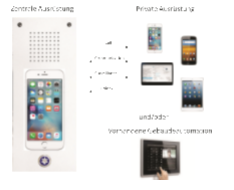
\includegraphics[height=8cm]{image/Titleimage.png}
	
	    \normalsize
	    \vspace{1cm}
	    \large \textbf{Bachelorarbeit}\\
	    \vspace{1cm}
	
	 \normalsize
	 	{
			\begin{tabular}{lll}
				\textbf{Studiengang:} & & Systemtechnik\\
				\textbf{Profil:} & & Informations- und Kommunikationssysteme\\
				\textbf{Referent:} & & Prof. Dr. Hauser-Ehninger Ulrich, MSc in Electronic Engineering\\
				\textbf{Korreferent:} & & Toggenburger Lukas, Master of Science FHO in Engineering\\
			\end{tabular}
	    }
    \end{center}
\end{titlepage}

\cleardoublepage
% \part im Inhaltsverzeichnis nicht nummerieren
\makeatletter
\let\partbackup\l@part
\renewcommand*\l@part[2]{\partbackup{#1}{}}

% leere Seite einfügen nach dem Titel
\thispagestyle{empty}
\quad 
\newpage

\pagenumbering{Roman}
\pagestyle{plain}
\section*{Zusammenfassung}
\label{sec:zusammenfassung}
%\addcontentsline{toc}{section}{Zusammenfassung}

Lorem ipsum dolor sit amet, consetetur sadipscing elitr, sed diam nonumy eirmod tempor invidunt ut labore et dolore magna aliquyam erat, sed diam voluptua. At vero eos et accusam et justo duo dolores et ea rebum. Stet clita kasd gubergren, no sea takimata sanctus est Lorem ipsum dolor sit amet. Lorem ipsum dolor sit amet, consetetur sadipscing elitr, sed diam nonumy eirmod tempor invidunt ut labore et dolore magna aliquyam erat, sed diam voluptua. At vero eos et accusam et justo duo dolores et ea rebum. Stet clita kasd gubergren, no sea takimata sanctus est Lorem ipsum dolor sit amet. Lorem ipsum dolor sit amet, consetetur sadipscing elitr, sed diam nonumy eirmod tempor invidunt ut labore et dolore magna aliquyam erat, sed diam voluptua. At vero eos et accusam et justo duo dolores et ea rebum. Stet clita kasd gubergren, no sea takimata sanctus est Lorem ipsum dolor sit amet.   

Duis autem vel eum iriure dolor in hendrerit in vulputate velit esse molestie consequat, vel illum dolore eu feugiat nulla facilisis at vero eros et accumsan et iusto odio dignissim qui blandit praesent luptatum zzril delenit augue duis dolore te feugait nulla facilisi. Lorem ipsum dolor sit amet, consectetuer adipiscing elit, sed diam nonummy nibh euismod tincidunt ut laoreet dolore magna aliquam erat volutpat.   

Ut wisi enim ad minim veniam, quis nostrud exerci tation ullamcorper suscipit lobortis nisl ut aliquip ex ea commodo consequat. Duis autem vel eum iriure dolor in hendrerit in vulputate velit esse molestie consequat, vel illum dolore eu feugiat nulla facilisis at vero eros et accumsan et iusto odio dignissim qui blandit praesent luptatum zzril delenit augue duis dolore te feugait nulla facilisi.   

Nam liber tempor cum soluta nobis eleifend option congue nihil imperdiet doming id quod mazim placerat facer

\section*{Abstract}
\label{sec:abstract}
%\addcontentsline{toc}{section}{Abstract}

In a world where everything is moving forward at the speed of light, home building technology is no exception. There are plenty of systems needed around building a house. One of them is the intercom.   
\\
\\
During our bachelor thesis, we developed a prototype for an intercom, based on open source software and hardware components. One of the aims of this project, was to evaluate and proof the ability of such components to handle this kind of application.
\\
During the design phase, many different requirements were defined. The intercom needed to be able to provide an audio and video stream. Nowadays everyone is always connected to the internet, thanks to the power of modern communication systems like Tablets and Smartphones. So, there was no doubt about the need of the intercom to be fully digital. As soon as things like digital real-time Video- and Audio transmissions comes on the table, also a lot of different complications and challenges comes with it too.
\\
\\
As a result, we came up with a prototype, that provides a flexible, up-to-date, and reasonably inexpensive solution for a modern house intercom system.

\newpage

% leere Seite einfügen
\thispagestyle{empty}
\quad 
\newpage
%%Inhaltsverzeichnis
\tableofcontents
\newpage

%%Seitennummerierung neu beginnen, Zahlen [arabic], röm.Zahlen [roman,Roman], Buchstaben [alph,Alph]
\pagenumbering{arabic}
\newpage
\pagestyle{fancy}

\definecolor{snippetcolor}{gray}{0.9}






%\section{Einleitung}
\label{sec:einleitung}

List Example:
\begin{itemize}
\item Maximaler Schub beim Starten z.B. wegen kurzer Startbahn
\item Maximale Fluggeschwindigkeit erreichen z.B. bei Rettungsflügen oder Ähnlichem
\item Maximale Effizienz z.B. um möglichst lange Flugzeiten zu ermöglichen
\end{itemize}



Bild Beispiel:
\vspace{0.05cm}

\begin{figure}[htb!]
	\begin{center}
		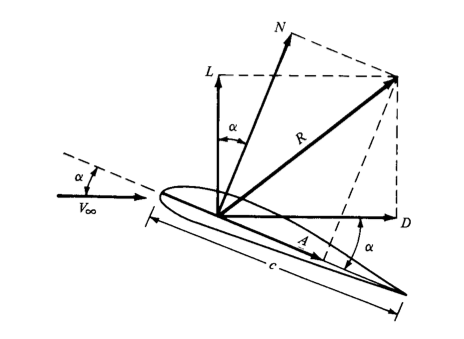
\includegraphics[width=0.48\textwidth]{airfoilKraefte}
		\caption[Wirksame aerodynamische Kräfte an einem Profil]{Wirksame aerodynamische Kräfte an einem Profil \cite{aeroKraefte}. Die Auftriebskraft $L$ wirkt beim Propeller als Schub und die Widerstandskraft $D$ als Drehmoment.}
		\label{fig:airfoilKraefte}
	\end{center}
\end{figure}

\vspace{0.05cm}

Unterkapittel:

\subsection{Subsection test}
\label{subsec:speichernderresultatematlab}

Wenn die Propellerberechnung beendet ist, werden alle Resultate in eine Baumstruktur gespeichert. Somit sind die Resultate schnell wieder aufrufbar und auch sauber in einer einzigen Datei geordnet und gespeichert.\\

\subsubsection{Subsubsection test}
\label{subsubsec:speichernderresultatematla2}

Wenn die Propellerberechnung beendet ist, werden alle Resultate in eine Baumstruktur gespeichert. Somit sind die Resultate schnell wieder aufrufbar und auch sauber in einer einzigen Datei geordnet und gespeichert.\\

\subsubsection{Subsubsubsection test}
\label{subsubsec:speichernderresultatematlab3}

Wenn die Propellerberechnung beendet ist, werden alle Resultate in eine Baumstruktur gespeichert. Somit sind die Resultate schnell wieder aufrufbar und auch sauber in einer einzigen Datei geordnet und gespeichert.\\

\newpage


%\section{Chapter Example}
\label{sec:chapterexample}


Um Berechnungen rund um das Thema Propeller durchführen zu können, ist es nötig, die sogenannte Blade- und Momentum-Theorie zu verstehen und diese anwenden zu können. Die Ausführungen in dieser Arbeit orientieren sich stark an der Master-Thesis von Mario Heene\cite{heene}. Ebenfalls werden die wichtigsten Begriffe der Aerodynamik und Propellertheorie erläutert. 
%\subsection{Underchapter Example}
\label{subsec:underchapterexample}

Die Gestalt von Propellern kann durch viele 2D-Profile beschrieben werden. 2D-Profile gleichen dem Querschnitt eines Flügels. Durch den geringeren Druck auf der Oberseite des Profils resultieren Kräfte, die das Profil hoch drücken (siehe Kapitel \ref{subsec:momentumtheorie}, Einschub Bernoulli) oder im Falle des Propellers, Schub erzeugen. Für jedes Profil können die Kräfte dargestellt werden.

\vspace{0.05cm}

\begin{figure}[htb!]
\begin{center}
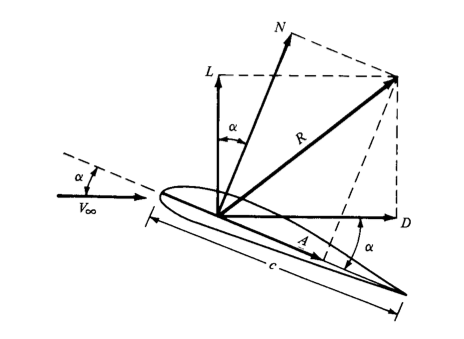
\includegraphics[width=0.48\textwidth]{airfoilKraefte}
\caption[Wirksame aerodynamische Kräfte an einem Profil]{Wirksame aerodynamische Kräfte an einem Profil \cite{aeroKraefte}. Die Auftriebskraft $L$ wirkt beim Propeller als Schub und die Widerstandskraft $D$ als Drehmoment.}
\label{fig:airfoilKraefte}
\end{center}
\end{figure}

\vspace{0.05cm}

In Abbildung \ref{fig:airfoilKraefte} sind die verschiedenen Kräfte dargestellt. $V_\infty$ stellt die Geschwindigkeit der Luft weit weg vom Körper dar. Die Kraft $R$ setzt sich zusammen aus der Auftriebskraft $L$ ('lift') und der Widerstandskraft $D$ ('drag'), wobei $L$ senkrecht zu $V_\infty$ steht und $D$ in die gleiche Richtung zeigt wie $V_\infty$.
Die Sehnenlänge $c$ ('chord') definiert die Länge des Profils von der Profilspitze bis zur Hinterkante. Dabei steht die Kraft $N$ senkrecht zu $c$ und $A$ in Richtung $c$. Der Winkel $\alpha$ ist der Winkel zwischen $V_\infty$ und $c$.
Über trigonometrische Funktionen können die Kräfte $N$ und $A$ folgendermassen beschrieben werden:

 

\section{Einführung}
\label{sec:chapterexample}

\subsection{Problemstellung}
\label{sec:chapterexample}

Heutzutage liefern diverse Hersteller verschiedene Lösungen für das Türglockensystem. Diese sind meistens Komplettsysteme, die nicht nur das einfache Klingel ermöglichen, sondern auch Zusatzfunktionen wie das Video-Streaming anbieten. Diese Systeme sind aber meistens proprietär und werden, gemäß Abschnitt \ref{sec:marktsituation},  für sehr hohe Preise verkauft.
\\
Die Komponenten, die für solche Systeme notwendig sind, sind aber heutzutage kostengünstig auf dem Markt erhältlich. Das Erarbeiten preiswerter Lösungen müsste somit möglich sein.
\\
Natürlich spielen die Kosten einer \gls{turklingelanlage} auf die Investitionen eines Neubaus keine so grosse Rolle. Sicher besteht aber in diesem Bereich eine Marktlücke und somit die Möglichkeit neue, bessere und günstigere Lösungen zu entwickeln.

\subsection{Grundidee}
\label{sec:grundidee}
Die Grundidee dieser Arbeit ist es, durch das Zusammenspiel verschiedener Systemen und Technologien, eine kostengünstige und funktionale \gls{turklingelanlage} zu entwickeln.
\\ 
Um den Kostenfaktor zu berücksichtigen, soll die Anlage auf schon vorhandene Technologien und Hardware basieren. Somit fallen die hohen Kosten für die Beschaffung proprietärer Hardware weg.
\\
In einer Zeit, in der die Hausautomation und das «Internet of things» immer mehr Bedeutung gewinnen, soll die \gls{turklingelanlage} diese Standards in Betracht ziehen. Dieses System soll den Benutzern ermöglichen, Ihre \gls{turklingelanlage} durch herkömmliche Smartphone oder Tablet zu bedienen.
\\
Klingelt ein Besucher an der Eingangstüre, soll der Wohnungsbesitzer über sein Smartphone darauf aufmerksam gemacht werden. Über eine am Eingang installierte Kamera  bekommt er auch die Möglichkeit den Besucher im Streaming zu sehen und die Türe, falls erwünscht, durch einen Handybefehl zu öffnen.
\newpage

\section{Projektplanung}
\label{sec:chapterexample}

\subsection{Prozess}
\label{sec:chapterexample}
Als Entwicklungsprozess wird ein hybrides Vorgehensmodell eingesetzt, welcher in Abbildung \ref{fig:hybridesModell} dargestellt wird. Im Rahmen einer Bachelorarbeit, in der die Anforderungen und Analysen schon im voraus im Fachmodul definiert worden sind, eignet sich am bestens ein lineares V-Modell. Ein solcher Prozess ist sehr schlank, übersichtlich und für diese Projektgrösse geeignet.
\\
Was das V-Modell nicht erlaubt, ist eine ständige Iteration mit dem Kunden während der Entwurf/Implementierungsphase. Daraus ergibt sich, wie im Abbild unten gezeigt, ein hybrides Modell welches uns zulässt, trotz der klar definierten Anforderungen, während der Entwurf- und der Implementierungsphase ein agiles Vorgehen mit dem Kunden durchzuführen.
\\
Die im Fachmodul geleistete Arbeit gehört zu den ersten zwei Phasen des Modells. Wie im linearen Vorgehensmodell vorgegeben, beginnt die nächste Phase der Arbeit sobald die vorherige Phase abgeschlossen ist. Die ganze Bachelorarbeit basiert auf Evaluationen und Entscheidungen, die in den ersten Phasen des Projekts getroffen worden sind. 

\begin{figure}[htb!]
	\begin{center}
		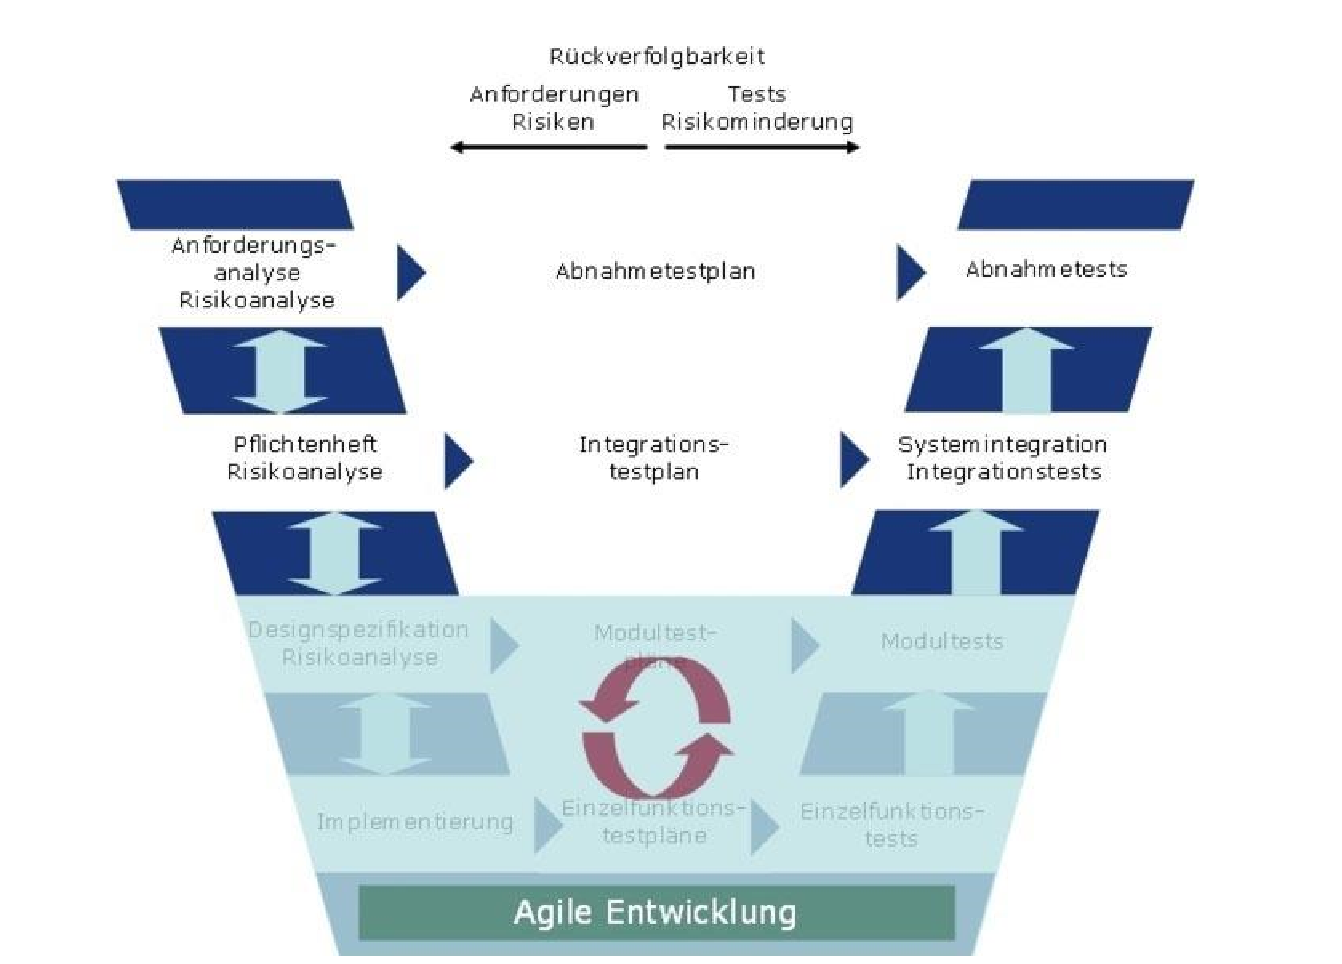
\includegraphics[width=0.89\textwidth]{hybridesModell}
		\caption[Hybrides Vorgehensmodell]{Hybrides Vorgehensmodell \\ (Quelle: https://www.eckelmann.de/en/services/development-process-models)}
		\label{fig:hybridesModell}
	\end{center}
\end{figure}


\subsection{Zeitplanung}
\label{sec:zeitplanung}
Die folgenden Abbildungen stellen die Projektplanung und die Meilensteine zeitlich dar (\seeref{fig:projektPlanungAchse} \& \cref{fig:projektPlanung}). In die erste Woche werden die Hardwarekomponenten, die mittlerweile schon bestellt wurden, getestet und zusammengebaut. 
\\
Die nächste zwei Hauptpunkte betreffen die Programmierung der  Software, die in zwei Teile geteilt wurde.
\\ 
Beim Teil 1 geht es um die Skripts die serverseitig kleine Aufgaben übernehmen, beim Teil 2 geht es um die Programmierung der Software. Da werden die Webapplikationen entwickelt, die auf den Aussensprechstellen und auf den mobilen Geräten der Bewohner ausgeführt werden sollen.
\\
Die letzte Phase ist für die Optimierung und als Reserve gedacht.

\begin{figure}[htb!]
	\begin{center}
		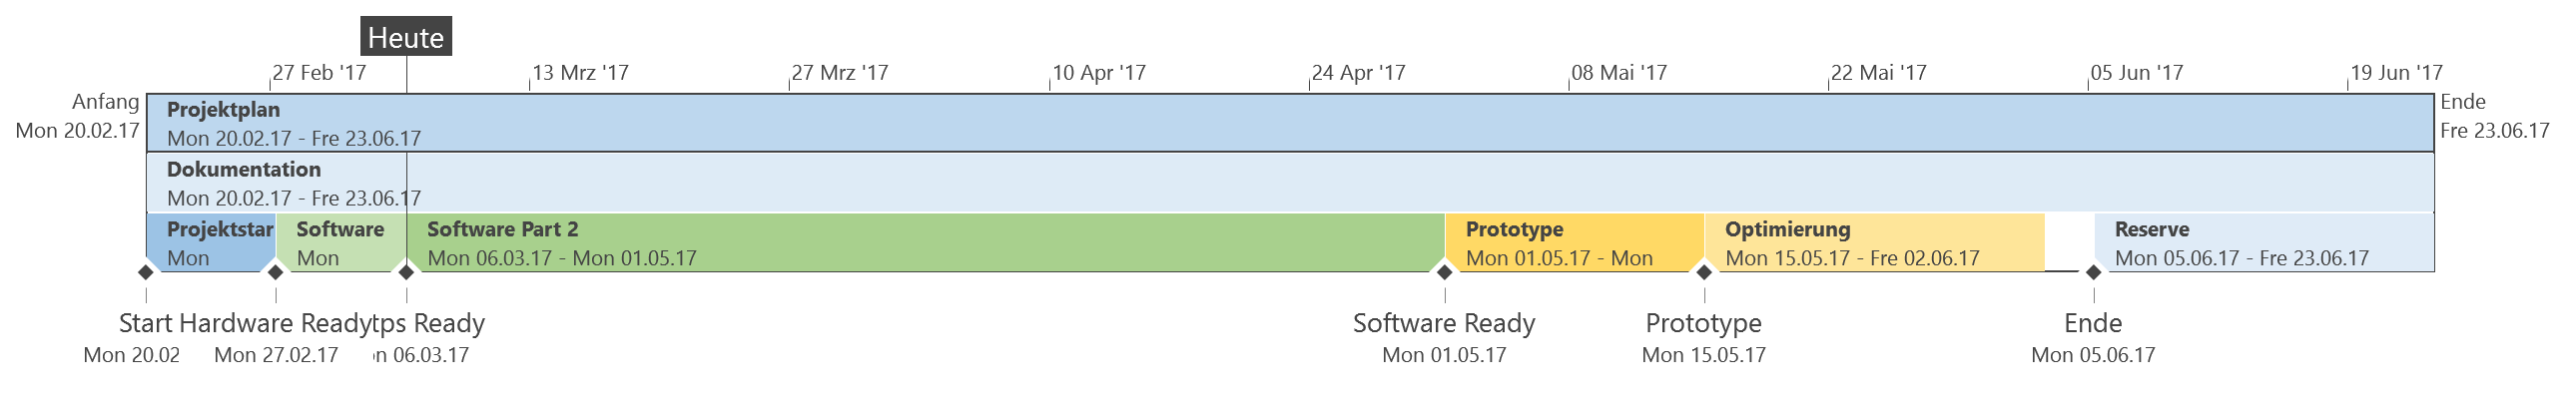
\includegraphics[width=1\textwidth]{projektPlanAchse}
		\caption[Projektplanung Meilensteine]{Zeitplanung mit Meilensteine}
		\label{fig:projektPlanungAchse}
	\end{center}
\end{figure}


\begin{figure}[htb!]
	\begin{center}
		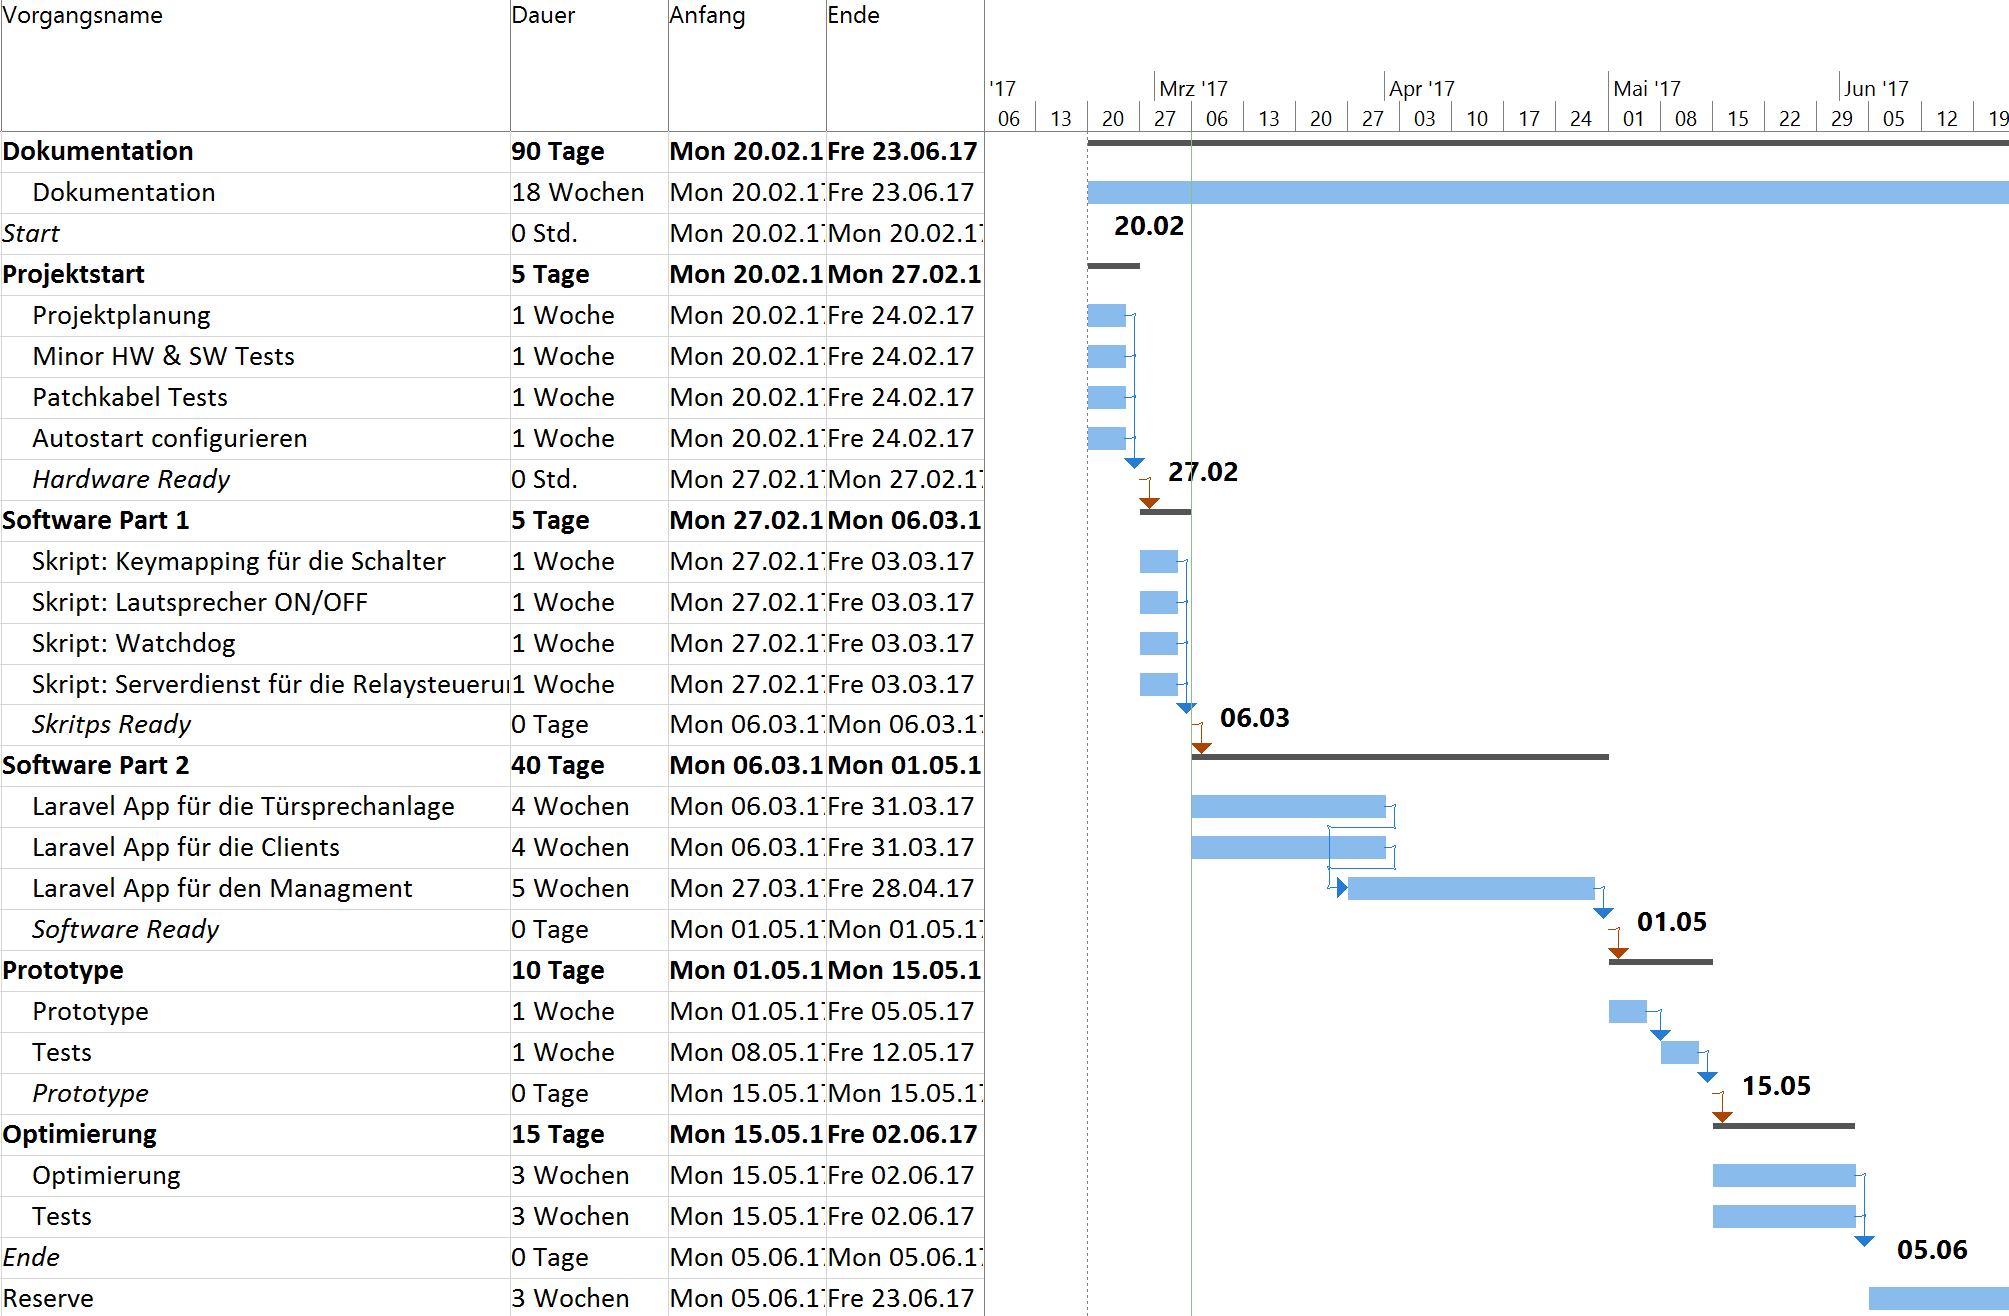
\includegraphics[width=0.9\textwidth]{projektPlanung}
		\caption[Projektplanung]{Projektplanung}
		\label{fig:projektPlanung}
	\end{center}
\end{figure}

\subsection{Versionierung}
Für die Versionierung und die gesamte Entwicklung wird das etablierte Open-Source Version-Control Software GIT verwendet. Das gesamte Quellcode, alle Bilder und Dokuemente werden in einem Repository gespeichert und versioniert.
\\
\\
Während die Entwicklung wird der Quellcode aber nicht Open-Source sein. Das Quellcode und die gesamte Entwicklungsdokumentation für das Projekt wird Vertraulich gehalten und nur für die Entwickler und Projektteilnehmer verfügbar sein. Für die Repository und das Backup wird also den Consumer Dienst Bitbucket verwendet.
\\
\\
Bitbucket (\seeref{fig:bitbucket}) ist ein webbasierter Filehosting-Dienst für Software-Entwicklungsprojekte, der die Versionsverwaltungssysteme Git und Mercurial unterstüzt. Bitbucket ermöglicht auch die Zusammenarbeit von mehreren Benutzern am gleichen Projekt. Bitbucket ist für ein Projekt dieser grosse kostenfrei.
\begin{figure}[htb!]
	\begin{center}
		
\includegraphics[width=1\textwidth]{bitbucket}
		\caption[Bitbucket ist ein Filehosting und ein Dienst für die Versionskontrolle von Softwareprojekte]{Bitbucket ist ein Filehosting und ein Dienst für die Versionskontrolle von Softwareprojekte}
		\label{fig:bitbucket}
	\end{center}
\end{figure}

\subsection{Risikoanalyse}
Inhalt der Risikoanalyse ist die frühzeitige Identifikation, das Bewerten von Problemen und das Definieren von Massnahmen die zu der Risikominimierung führen.
\\
Der Risiko-Management Prozess nach ISO 31000:2009 umfasst folgende Hauptpunkte: 

\begin{itemize}
	\item Risikoidentifikation: Liefert eine Liste von möglichen Risiken die während der Implementierungsphase auftreten könnten. 
	\item Aufgrund der Risikoidentifikation werden Zusammenhänge zwischen den Risiken und die Auswirkungen auf dem Projekt beurteilt. 
	\item Risikobewertung: Zu jedem Risiko werden die Eintrittswahrscheinlichkeit sowie die Auswirkung auf das Gesamtprojekt abgeschätzt.
	\item Risikobewertung: Zu jedem Risiko werden die Eintrittswahrscheinlichkeit sowie die Auswirkung auf das Gesamtprojekt abgeschätzt.
	\item Risikosteuerung: Maßnahmen planen, um die gemessenen und analysierten Risiken zu steuern.
\end{itemize}

\subsubsection{Identifikation Analyse und Bewertung}
Die Identifikation der Risiken erfolgte durch Brainstorming, aber auch durch Probleme die während den Sitzungen und der Projektplanerfassung aufgetaucht sind.
\\
\\
Um die aufgelisteten Risiken zu bewerten, wurde eine Risikomatrix eingesetzt. Diese soll eine visuelle Darstellung von Risikobewertungen geben. 
\begin{figure}[htb!]
	\begin{center}
		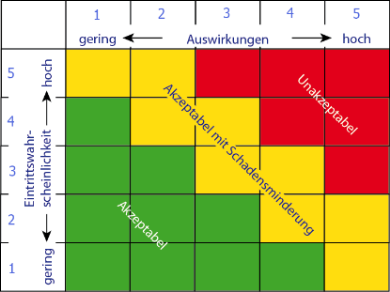
\includegraphics[width=0.5\textwidth]{risikomatrix}
		\caption[Risikomatrix]{Risikomatrix}
		\label{fig:risikomatrix}
	\end{center}
\end{figure}
\\
Die Auswirkungen sowie die Eintrittswahrscheinlichkeit werden mit einem Index (0 bis 5) von gering bis hoch eingestuft. Das Risiko ergibt sich durch die Multiplikation der beiden Achsen. Die Risiken die sich im roten Bereich der Matrix befinden, müssen bei der Risikosteuerung/Maßnahmen sehr intensiv und detailliert behandelt werden, damit einer der beiden Faktoren minimiert werden kann. 
\\
\subsubsection{Bewertung Projekt Risiken}
Die folgende Tabellen stammen aus dem Fachmodul.
\begin{figure}[htb!]
	\begin{center}
		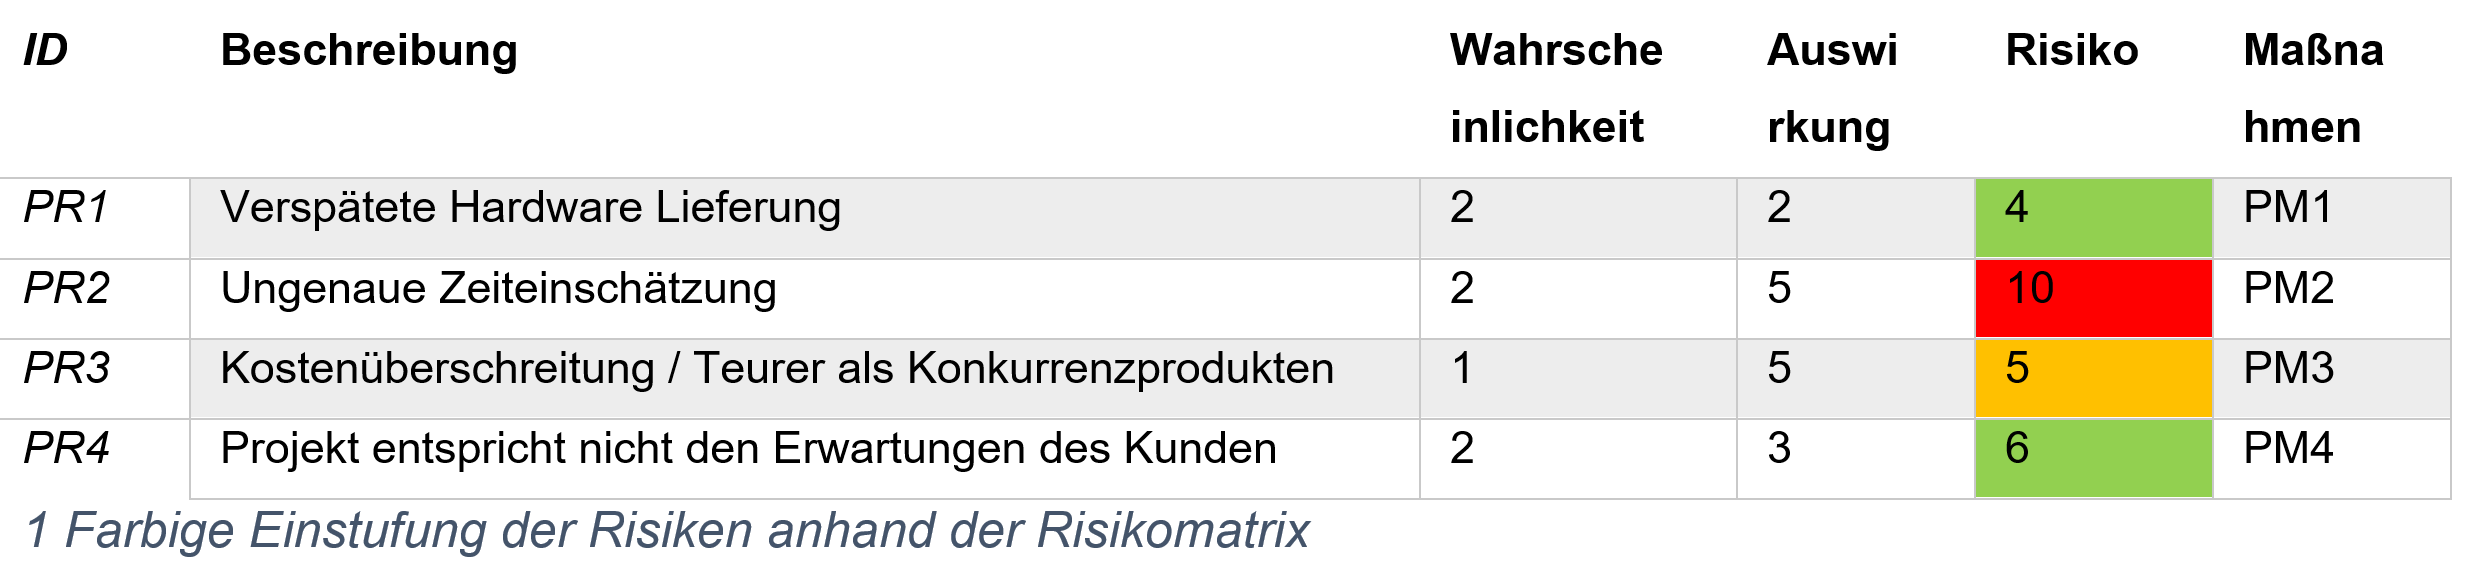
\includegraphics[width=0.95\textwidth]{projektrisiken}
		\caption[Bewertung Projekt Risiken]{Bewertung Projekt Risiken}
		\label{fig:projektrisiken}
	\end{center}
\end{figure}
\subsection{Bewertung Technische Risiken}
\begin{figure}[htb!]
	\begin{center}
		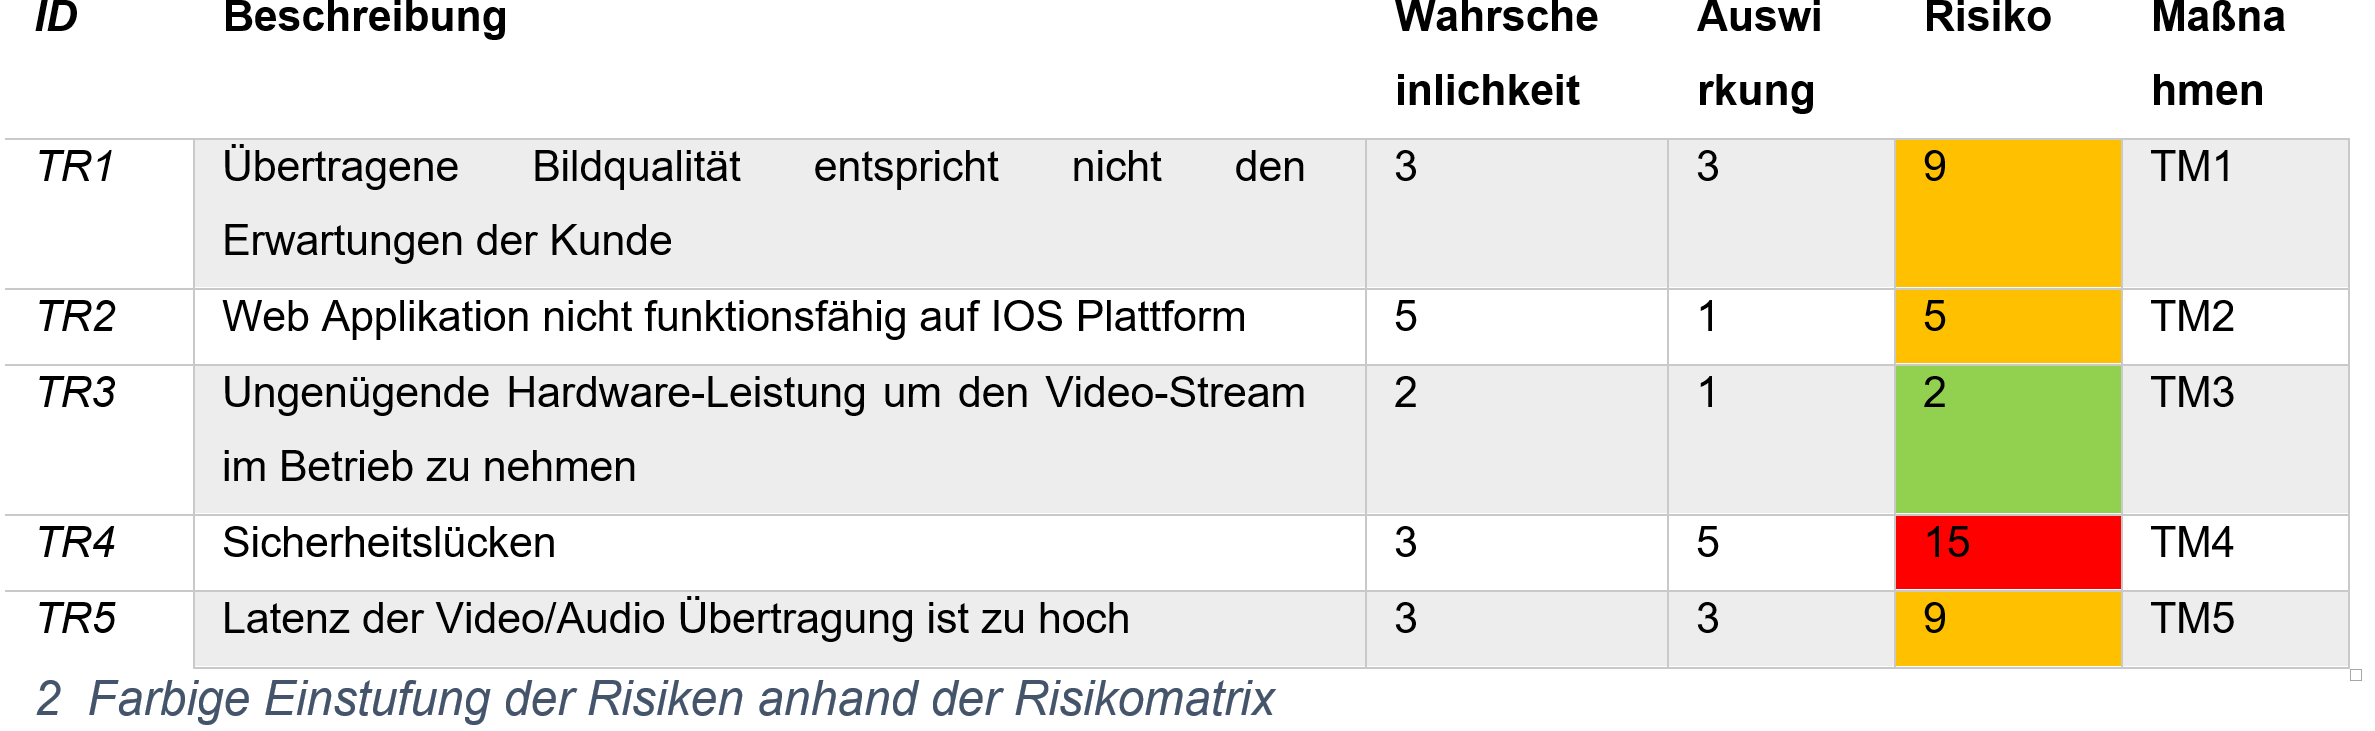
\includegraphics[width=0.9\textwidth]{bewertungrisiko}
		\caption[Bewertung Technische Risiken]{Bewertung Technische Risiken}
		\label{fig:techrisiko}
	\end{center}
\end{figure}
\subsubsection{Risikosteuerung \& Projekt Massnahmen}
\begin{figure}[htb!]
	\begin{center}
		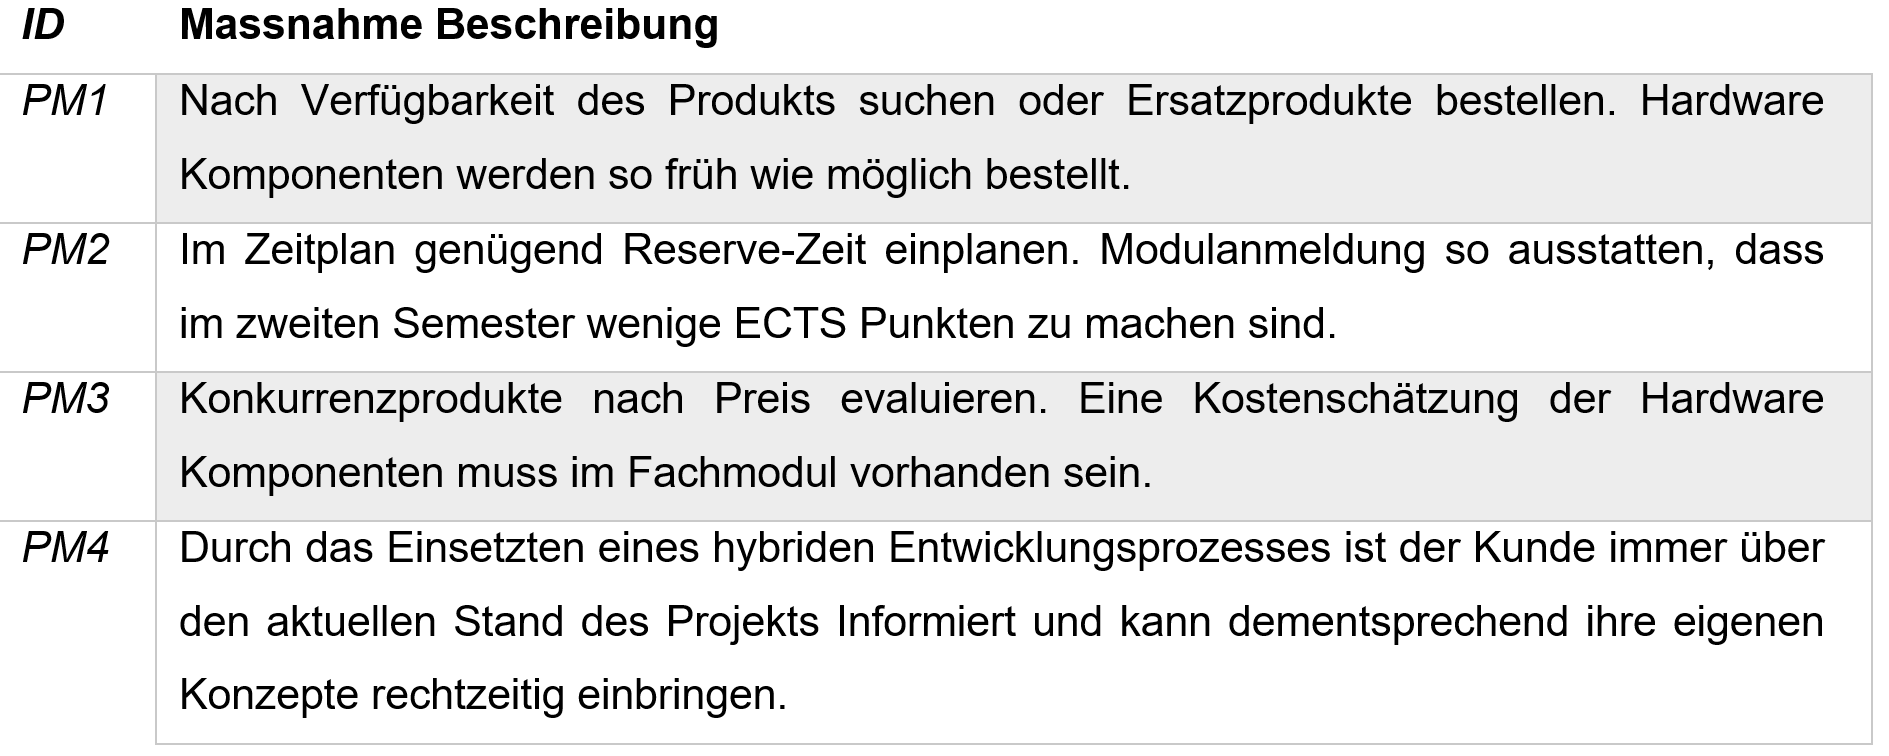
\includegraphics[width=0.75\textwidth]{massnahmen}
		\caption[Projekt Massnahmen]{Projekt Massnahmen}
		\label{fig:risikomassnahmen}
	\end{center}
\end{figure}

\newpage

\section{Aktueller Stand}
\label{sec:chapterexample}

Eine Türsprechanlage, welche Audio und Video überträgt ist keine neue Erfindung. Auf dem Markt existieren bereits verschiedene Lösungen und das schon seit mehreren Jahren. Diese sind aber meistens Analoge Systeme und verfügen über die Vorteile der Digitalisierung nicht. Die Steuerung über eine Mobileapplikation ist bei solche Lösungen aus diesem Grund ausgeschlossen.

\begin{figure}[htb!]
	\begin{center}
		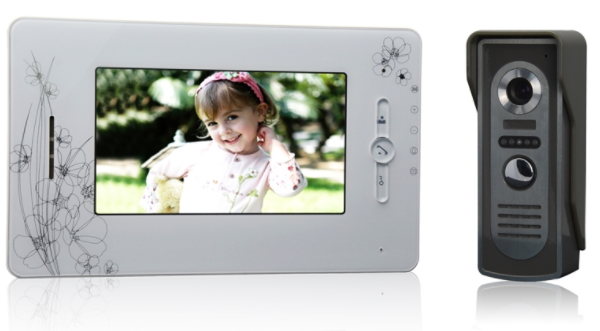
\includegraphics[width=0.66\textwidth]{analog_intercom}
		\caption[Analoge Türsprechanlage mit In-House Display]{Analoge Türsprechanlage mit In-House Display}
		\label{fig:analoge_intercom}
	\end{center}
\end{figure}

In den letzten Jahren sind die ersten Digitale Lösungen mit IP Videoübertragung auf dem Markt gekommen. Die Digitalisierung in diesem Bereich hat es die gigantische Schritten im Bereich der Miniaturisierung und die immer schnellere Internet Zugänge (xDSL, LTE, usw) zu verdanken.

\subsection{Die Herausforderungen der Digitalisierung}
Die Digitalisierung bringt nicht nur Vorteile mit sich. Besonders bei der Video und Audioübertragung. Während eine Analoge Videoübertragung ziemlich mühelos erfolgt muss im Fall eine Digitale Lösung das Video zuerst kodiert und dann dekodiert werden.
\\
Die heutige Kodierung-Algorithmen ermöglichen eine ziemlich schnelle Dekodierung. Mittlerweile hat jeder Smartphone genug Leistung um ein Full-HD Videostream vom Youtube oder Netflix in real-time zu dekodieren. Auf die andere Seite ist die Kodierung ein sehr rechenintensiven Prozess und benötigt sehr viel Leistung.
\\
Jeder der schon mal mit Video-Editing zu tun hatte, weisst, wie viel Zeit die Exportierung eines Video dauern kann.
\\
Die grösste Herausforderung für die real-time Digitale Video/Audio Kommunikation besteht also darin, die Kodierung und Dekodierung der Audio und Video Signal im vernünftigen Zeit durchzuführen. 

\subsection{Marktsituation}
\label{sec:chapterexample}
Der Hauptziel dieses Bachelorarbeit ist, eine Kostengünstige Lösung für eine digitale, flexible und skalierbare Gegensprechanlage. Tatsächlich ist es so, dass die bestehende Lösungen sehr teuer sind. Viele Produkte basieren auf Drittanbieter, SIP Gateways oder andere Elemente die Zusatzkosten verursachen. Das möchten wir alles vermeiden.

\begin{figure}[htb!]
	\begin{center}
		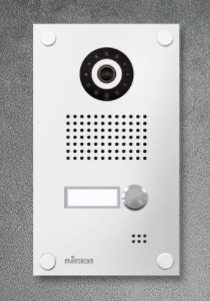
\includegraphics[width=0.33\textwidth]{myintercom}
		\caption[Telecom Behnkle MyIntercom]{Telecom Behnkle MyIntercom}
		\label{fig:myintercom}
	\end{center}
\end{figure}

Eine der günstigsten Produkte den wir finden konnten ist das \textit{"MyIntercom"} von Telecom Behnkle (\seeref{fig:myintercom}). Diese Türklingelanlage ist ziemlich flexibel und bietet die Möglichkeit, mehrere Türen anzuschliessen. Der Preis liegt hier bei zirka 1'600.- CHF pro Türe bei dem Basic-Modell.
\\
\\
 Dank der Aufschwung von Open-Source Hardware wie das Raspberry PI und Real Time Communication Protokolle wie WebRTC muss es möglich sein, kostengünstigere Lösungen zu erarbeiten. Bei den folgenden Kapiteln geht es nun um die effektive Realisierung einem Prototyp, welches die oben genannte Problemen adressiert. 

\newpage
\section{Anforderungen}
Für den Bachelorarbeit wurden die Anforderungen bereits in dem Fachmodul definiert.
\subsection{Anforderungen}
A1. Es soll möglich sein, die Haustüre durch ein Signal zu öffnen. 
\\
\\
A2. Es soll möglich sein, ein Videosignal von der Aussensprechstelle zum Client zu streamen. 
\\
\\
A3. Es soll möglich sein, ein Audiosignal zwischen der Aussensprechstelle und der Client App bidirektional zu streamen. 
\\
\\
A4. Ein digitaler Bildschirm zeigt die Informationen der Bewohner (Name, Vorname, usw) an der Aussensprechstelle an. 
\\
\\
A5. Nach einem Stromunterbruch soll die Anlage automatisch wieder Starten und Funktionsbereit sein. 
\\
\\
A6. Den Datenverkehr zwischen den Endknoten muss Verschlüsselt sein. 
\\
\\
A7. Die Komponenten sollten zwischen -20C und +40C funktionsfähig sein. 
\\
\\
A8. Die Komponenten sollten auch im Fall hoher Feuchtigkeit funktionsfähig sein. (80\%) 
\\
\\
A9. Die Kamera für das Videosignal muss eine Auflösung von mind. 1280x720 Pixel aufweisen.  
\\
\\
A10. Die Materialkosten pro Aussensprechstelle sollten 400.- nicht überschreiten. 
\\
\\
A11. Die Aussensprechstelle soll auch mit nasse/bedeckte Hände bedienbar sein. 
\\
\\
A12. Bei der Innenstelle ist es möglich das Mikrofon auszuschalten, um die Übertragung des Audiosignales zu unterdrücken. 

\subsection{Wunschanforderungen}
W1. Die Komponenten sollten die Speisung durch PoE erhalten. 
\\
\\
W2. Die Kamera für das Videosignal muss eine Auflösung von 1920x1080 Pixel aufweisen. 
\\
\\
W3. Verpasste Besuche sollten aufgezeichnet werden und in der Client App in Form von einem Foto und Notifikation sichtbar sein.
\newpage

\section{Lösungskonzept}
\label{sec:lösungskonzept}
Die \cref{fig:hwoverview} zeigt einen Überblick über die verschiedenen Hardwarekomponenten, die für die \gls{turklingelanlage} benötigt werden.
\\
Es werden nun zwei Begriffe erklärt, die in diesem Dokument von grosse Bedeutung sind. Das erste ist die \gls{turklingelanlage}. Damit gemeint ist die Gesamtheit der Komponenten die denn Zusammen den Endprodukt darstellen.
\\
Als \gls{aussensprechstelle} ist die Gesamtheit aller Komponenten des Endproduktes gemeint, als Aussensprechstelle der an der Eingangstüre installierte Mikrocontroller inklusive dazugehörige Module.
\\
Räumlich von der \gls{aussensprechstelle} getrennt befindet sich der Server. Dieser besteht aus einem Mikrocontroller, der als Server im Einsatz steht, aus einem Switch der dazu dient die \gls{aussensprechstelle} mit Strom und Datenverbindung zu versorgen und aus einem Relais welches den Türöffner und die Glocke betätigt.
\begin{figure}[htb!]
	\begin{center}
		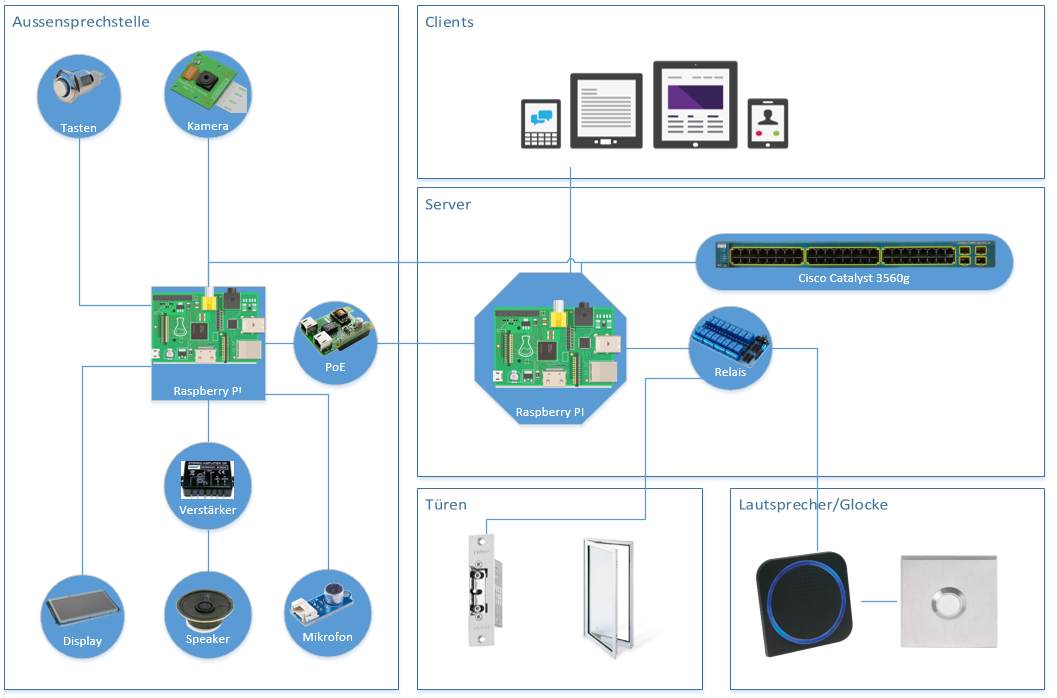
\includegraphics[width=0.95\textwidth]{hwoverview}
		\caption[Hardware Ecosystem]{Hardware Ecosystem}
		\label{fig:hwoverview}
	\end{center}
\end{figure}
Das System besteht aber nicht nur aus Hardware. Das Zusammenarbeiten der Hardware wird von viel Softwareelemente geregelt. Als erstes, wie bereits in der Projektplanung definiert, wird die Hardwareseite der Lösung realisiert. Sobald alle Hardwarekomponenten getestet und auf Kompatibilität geprüft worden sind, wird die Programmierung stattfinden.
\newpage

\section{Umsetzung der Hardware}
\label{sec:chapterexample}
\subsection{Komponenten}
Das System wird hardwareseitig grob in zwei Teile unterteilt, den Server und die \gls{aussensprechstelle}.
\\
Die \cref{tbl:SrvHW} und die \cref{tbl:DoorHW} zeigen die benötigten Hardwarekomponenten, welchen an den jeweiligen Stellen eingebaut werden.
\\
Um den Überblick über die Kosten aller Hardwarekomponenten zu behalten, sind hier auch die Preisen aufgelistet. Dabei ist es wichtig sicherzustellen, dass die gesamten Hardwarekosten diejenigen der von der Konkurrenz angebotenen Produkte nicht übersteigen.
\\
Die Einkaufspreise sind nur Richtpreise, da es sich um Standardkomponenten handelt und die Marktpreise sich ständig und schnell ändern können. Die Summen sind als Kostenschätzung zu betrachten. (Stand Fruhjahr 2017).

\begin{table}[]
	\centering
	\label{my-label}
	\begin{tabular}{l|ll}
		\multicolumn{1}{r|}{} \textbf{Anzahl} & \textbf{Komponente} \hspace{180pt} & \textbf{Preis} 	\\ \hline
		1	&	Raspberry Pi 3 Model B						& 50.-				\\ \hline
		1	&	Raspberry Gehäuse und Netzteil				& 25.-			\\ \hline
		2	&	8-Kanal Relais Modul						& 15.-			\\ \hline
		1	&	\textit{Kleinmaterial}						& 15.-			\\ \hline
		\textbf{Total}	&									& \textbf{140.-}			\\ \hline
	\end{tabular}
	\caption{Server \gls{hw} Komponenten}
	\label{tbl:SrvHW}
\end{table}

\begin{table}[]
	\centering
	\label{my-label}
	\begin{tabular}{l|ll}
		\multicolumn{1}{r|}{} \textbf{Anzahl} & \textbf{Komponente} \hspace{180pt} & \textbf{Preis} 	\\ \hline
		1	&	Raspberry Pi 3 Model B		   				& 50.-			\\ \hline
		1	&	4" Bildschirm								& 64.-			\\ \hline
		1	&	Raspberry Kamera							& 59.-			\\ \hline
		1	&	\gls{poe} Adapter									& 50.-			\\ \hline
		3	&	Schalter									& 25.-			\\ \hline
		1	&	Mikrophon									& 12.-			\\ \hline
		1	&	Lautsprecher								& 9.-			\\ \hline
		1	&	Audio Verstärker							& 10.-			\\ \hline
		1	&	\textit{Kleinmaterial / Gehäuse}			& 50.-			\\ \hline
		\textbf{Total}	&									& \textbf{329.-}			\\ \hline
	\end{tabular}
	\caption{Aussensprechstelle \gls{hw} Komponenten}
	\label{tbl:DoorHW}
\end{table}

\subsection{Stromspeisung}
\label{sec:poe}
Ein Ziel unserer Lösung ist die Installationskosten zu senken und die Montage zu vereinfachen. Aus diesem Grund war für unsere Lösung wichtig, \gls{poe} zu verwenden. In modernen Haushalte werden meistens Ethernet Verkabelungen verlegt und dank PoE ist nur noch ein Kabel, welches Strom und Konnektivität gewährleistet, notwendig.
\\
\\
Zusätzlich benötigt das System noch eine Leitung die den Türöffner steuert.
Auch diese Endinstallation kann vereinfacht werden wenn man, anstatt ein dediziertes Kabel zwischen Server und Türöffner einzuziehen,  zwei Drähte des bereits installierten Ethernet Kabels verwendet.
\\
\\
Cisco Catalyst 3560g welcher für den \gls{poe} Stromversorgung zuständig ist, verwendet die Phantomspeisung oder Mode A. Das heisst, dass die mit der Datenübertragung belegten Drähte mit der Stromversorgung überlagert werden. Dies ist möglich da die Frequenz der Elektrizität 60 Hz beträgt und die der Datenübertragungen im Bereich von 10-100MHz liegt.

\begin{figure}[htb!]
	\begin{center}
		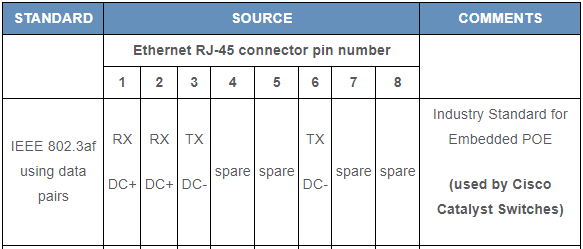
\includegraphics[width=0.89\textwidth]{CatalystPoEpinouts}
		\caption[Catalyst Pinouts]{Catalyst 3560g \gls{poe} Pinbelegung}
		\label{fig:catalystPinouts}
	\end{center}
\end{figure}

Wie im \cref{fig:ethernetBelegung} dargestellt werden die Adern 7 und 8 dazu verwendet um den Türöffner zu betätigen. Aus den 3 verbliebenden Adernpaaren kann maximal die Ethernetkategorie 100BASE-T erreicht werden. Da aber \gls{webrtc} eine erhebliche kleinere Bandbreite in Anspruch nimmt, stellt es für die \gls{aussensprechstelle} kein Hindernis dar.

\begin{figure}[htb!]
	\begin{center}
		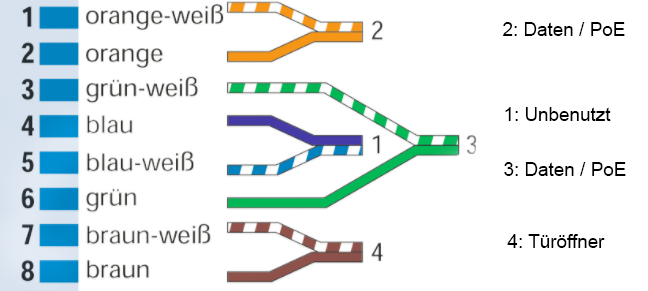
\includegraphics[width=0.89\textwidth]{EthernetPinbelegung}
		\caption[EthernetPinbelegung]{Cat. 7 Ethernet Pinbelegung der \gls{aussensprechstelle}}
		\label{fig:ethernetBelegung}
	\end{center}
\end{figure}



\subsection{Server}
\label{sec:chapterexample}
Der Server wird mit einem Relais-Board verbunden um die Gongs und die Türöffner zu bedienen. An dieser Stelle ist die Hardwarekonfiguration sehr einfach. Mit der aktuellen Hardwarekonfiguration könnten bis 8 Wohnungen und 8 Aussensprechstellen angeschlossen werden. Die \cref{fig:pipins} und die \cref{fig:boardpins} zeigen die Pinbelegung auf dem Pi und auf dem Relais-Board. Die \cref{tbl:pinroutes} zeigt wie die verschiedenen Pins miteinander verbunden werden.

\begin{figure}[htb!]
	\begin{center}
		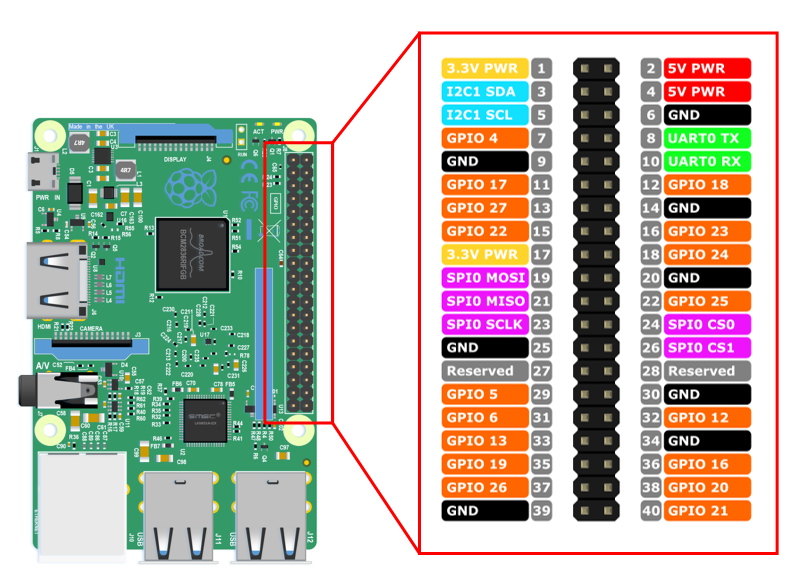
\includegraphics[width=0.8\textwidth]{pipins}
		\caption[EthernetPinbelegung]{Pinbelegung der \gls{aussensprechstelle}}
		\label{fig:pipins}
	\end{center}
\end{figure}

\begin{figure}[htb!]
	\begin{center}
		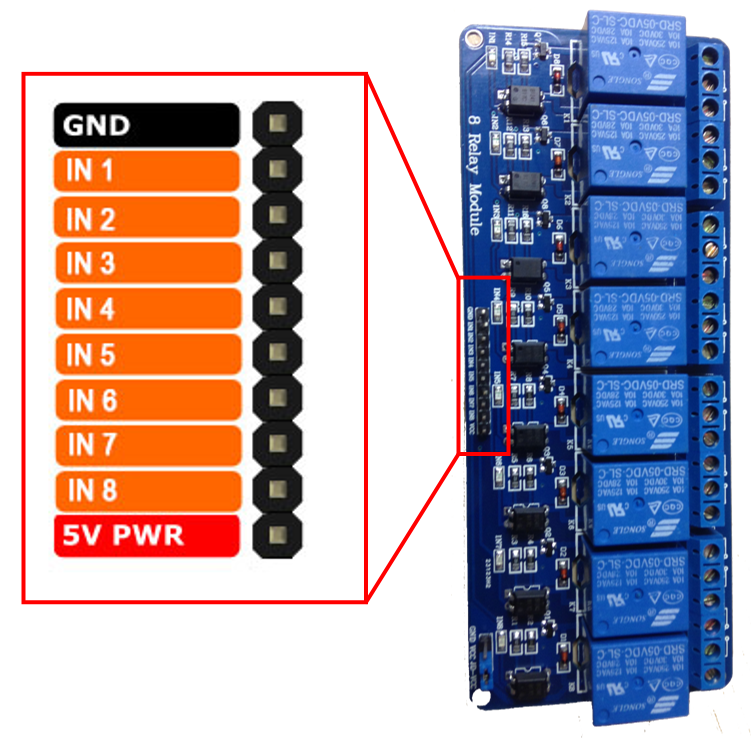
\includegraphics[width=0.55\textwidth]{boardpins}
		\caption[EthernetPinbelegung]{Pinbelegung für das Relais-Modul}
		\label{fig:boardpins}
	\end{center}
\end{figure}

\begin{table}[]
	\centering
	\label{my-label}
	\begin{tabular}{l|ll}
		\multicolumn{1}{r|}{} \textbf{Pi GPIO (PIN)} & \textbf{Relais IN (Board Nr)} & \textbf{Funktion}  \hspace{60pt}	\\ \hline
		GPIO4 (7)	&	IN1 (1)			& Gong WG.1			\\ \hline
		GPIO17 (11)	&	IN2 (1)			& Gong WG.2			\\ \hline
		GPIO27 (13)	&	IN3 (1)			& Gong WG.3			\\ \hline
		GPIO22 (15)	&	IN4 (1)			& Gong WG.4			\\ \hline
		GPIO5 (29)	&	IN5 (1)			& Gong WG.5			\\ \hline
		GPIO6 (31)	&	IN6 (1)			& Gong WG.6			\\ \hline
		GPIO13 (33)	&	IN7 (1)			& Gong WG.7			\\ \hline
		GPIO19 (35)	&	IN8 (1)			& Gong WG.8			\\ \hline
		GPIO18 (12)	&	IN1 (2)			& Türöffner Türe 1			\\ \hline
		GPIO23 (16)	&	IN2 (2)			& Türöffner Türe 2			\\ \hline
		GPIO24 (18)	&	IN3 (2)			& Türöffner Türe 3			\\ \hline
		GPIO25 (22)	&	IN4 (2)			& Türöffner Türe 4			\\ \hline
		GPIO12 (32)	&	IN5 (2)			& Türöffner Türe 5			\\ \hline
		GPIO16 (36)	&	IN6 (2)			& Türöffner Türe 6			\\ \hline
		GPIO20 (38)	&	IN7 (2)			& Türöffner Türe 7			\\ \hline
		GPIO21 (40)	&	IN8 (2)			& Türöffner Türe 8			\\ \hline
	\end{tabular}
	\caption{PIN-Zuweisung zwischen den Server und die Relais Module}
	\label{tbl:pinroutes}
\end{table}


\subsection{Aussensprechstelle}
\label{sec:chapterexample}
Bei der \gls{aussensprechstelle} wird auch ein Raspberry Pi eingesetzt. Hier sind mehrere Zusatzkomponenten notwendig. Die Speisung, wie oben schon erwähnt, erfolgt an dieser Stelle über \gls{poe}. Aus diesem Grund ist ein \gls{poe}-Splitter vorhanden.
\\
Für die Audiowiedergabe sind ein kleiner Lautsprecher und ein Verstärker notwendig. Der Chinch Anschluss des Raspberrys Pi hat eine zu niedrige Ausgangsleistung um den Lautsprecher direkt anschliessen zu können.
\\
Die drei Schalter, die für die Bedienung der \gls{aussensprechstelle} notwendig sind, werden an die \gls{gpio}s des Raspberrys PI angeschlossen. Die \cref{tbl:pinroutesdoor} zeigt die Pinbelegung.

\begin{table}[]
	\centering
	\label{my-label}
	\begin{tabular}{l|ll}
		\multicolumn{1}{r|}{} \textbf{Pi GPIO (PIN)} & \textbf{Schalter} & \textbf{Funktion} \hspace{60pt}	\\ \hline
		GPIO16 (36)	&	Schalter Links		&	Nach Links Scrollen	\\ \hline
		GPIO20 (38)	&	Schalter Mitte		&	Glocke läuten		\\ \hline
		GPIO21 (40)	&	Schalter Rechts		&	Nach Rechts Scrollen		\\ \hline
	\end{tabular}
	\caption{PIN-Zuweisung zwischen den Raspberry PI und die Schalter}
	\label{tbl:pinroutesdoor}
\end{table}

\subsubsection{Problemen}
Während der Zusammenstellung der Aussensprechstelle sind die erste unvorhergesehene Problemen aufgetaucht. Die Audiowiedergabe und Audioaufnahme stellten eine grössere Herausforderung als geplant dar.
\\
\\
\textbf{Audiowidergabe} 
\\
Die grösste Problematik bei der Audiowiedergabe besteht darin, dass die Massen des Raspberrys Pi, des Verstärkers und des Audio-Interface gekoppelt sind. Das führt zu Brummschleifen, die wiederum Störsignale auf dem Audio-Ausgang erzeugen. Um das zu vermeiden, muss an dieser Stelle ein Massentrennfilter eingesetzt werden.
\\
Die Störsignale sind nun fast komplett verschwunden, nur ein winziges Hintergrundgeräusch ist immer noch vorhanden. Um dieses Problem umzugehen, wird ein zusätzliches Relais installiert, welches den Lautsprecherstromkreis bei Nichtnutzung unterbricht.
\\
\\
\textbf{Das Mikrophon}
\\
Das Problem der Audioaufnahme liegt beim Mikrophon selber. Der Raspberry Pi besitzt kein integriertes Audio-Input. Aus diesem Grund wurde ein \gls{usb}-Audio-Interface verwendet. Es hat sich aber herausgestellt, dass es nicht so einfach ist, kostengünstige und qualitatives \gls{usb} Mikrophone zu finden. Die meisten Produkten sind nicht für den Outdoorbetrieb gedacht und oft ist die Empfindlichkeit zu gering um ein qualitatives Audiosignal aufzunehmen.  Für unseren Prototyp wird das eingesetzte Mikrophon völlig ausreichen, für ein gut funktionierendes Endprodukt sollte man ein besseres Mikrophon einbauen.
\newpage
\section{Software}
\label{sec:chapterexample}

\subsection{Programmiersprachen}
Das System besteht aus mehrere Programme und Dienste. Für die Entwicklung werden folgende Programmiersprachen eingesetzt:
\begin{itemize}
	\item Java
	\item Javascript
	\item PHP
\end{itemize}
Im Verbindung mit PHP kommt natürlich die Markup-Languages HTML5/CSS, welche für die graphische Darstellung der Webapplikationen notwendig ist.

\subsubsection{Java}
\label{kap:java}
Alle Dienste die Serverseitig und ohne Interaktion mit dem Enduser ausgeführt werden, werden in Java programmiert. Als stark typisierte und Objektorientierte Programmiersprache eignet sich Java für dieses Projekt. Für Java sind auch unzählige Libraries verfügbar, insbesondere für die Hardware Steuerung der Raspberry Pi. Eine zweite Variante wäre Python gewesen, die auch das Raspberry sehr gut unterstüzt. Python ist aber zu wenig typisiert und für eher kleinere Softwarestücke gedacht.

\subsubsection{PHP/Javascript}
Die Client Applikation sowohl auch die Applikation bei der Aussensprechstelle werden Web-Applikationen sein. Dies ermöglicht eine schnelle und zeitgemässe Softwareentwicklung. Für dieses Projekt ist die System-Eingriffstiefe von Webapplikationen jedenfalls ausreichend. Es muss lediglich Zugriff auf Mikrofon, Lautsprecher und Kamera garantiert werden. Ein weiteres Punkt zugunsten einer Webapplikation ist die Cross-Plattform Kompatibilität.
\\
Aus diesem Grund haben wir uns für PHP (Objektorientiert) im Kombination mit Javascript/HTML/CSS entschieden. Eine zweite Variante wäre Java EE gewesen. Java EE eignet sich aber vor allem für grosse Softwarelösungen und bietet als gesamten Framework vieles mehr als was dieses Projekt benötigt.
\\
\subsubsection{PHP Framework: Laravel}
Für die Entwicklung der Webapplikationen wird Laravel als PHP Framework eingesetzt. Laravel ist ein Open-Source PHP Web-Application-Framework, die sich für kleine bis zu mittelgrosse Projekte eignet. Laravel beruht auf dem Modell-View-Controller-Muster und ermöglicht eine Objektorientierte Programmierung in PHP.

\subsection{System Übersicht}
Das System besteht aus mehrere Hardware- und Softwarekomponenten die zusammenarbeiten müssen (\seeref{fig:echosystem}). Die  Vertraulichkeit der Kommunikation zwischen den Knoten ist von TLS immer gewährleistet. Die einzelne Komponenten, sowie das Thema Sicherheit, werden in den nächsten Kapiteln genauer beschrieben.

\begin{figure}[htb!]
	\begin{center}
		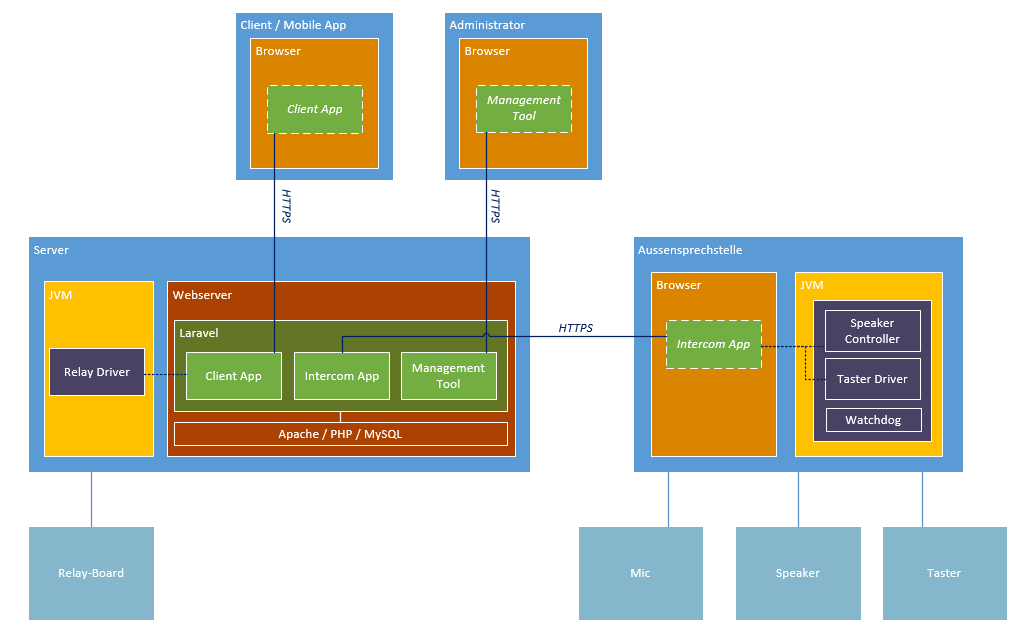
\includegraphics[width=1\textwidth]{ecosystem}
		\caption[Software / Hardware Ecosystem]{Software / Hardware Ecosystem}
		\label{fig:echosystem}
	\end{center}
\end{figure}

Die Software wird in zwei Gruppen unterteilt. Einerseits gibt es alle Dienste/Daemons \textit{(Violett)} die Lokal ausgeführt werden und quasi das Backend des Systems darstellen.
\\
Die zweite Gruppe beinhaltet die Webapplikationen \textit{(Grün)}, die eine GUI besitzen und für die Interaktion mit dem System gedacht sind. Darunter zählen die Client-App für den Bewohner, die Applikation bei der Aussensprechstelle wo die Bewohner angezeigt werden und das Management Tool.
\\
Die Audio/Video-Kommunikation zwischen die Aussensprechstellen und die Client-Apps wird mithilfe von WebRTC realisiert. Diese hat eine gewisse Komplexität und wird in ein eigenes Kapitel (\seeref{kap:webrtc}) behandelt.

\subsection{Raspbian}
\label{kap:raspbian}
Auf alle Raspberry Pi wurde den Betriebssystem Raspbian Jessie installiert. Diese wird von Raspberry Pi Foundation mitgeliefert und gilt als besonders hochoptimerte OS für die mit niedriger Leistung und geringem Stromverbrauch ARM Prozessoren.
Raspbian basiert auf Debian welche unter der DFSG (Debian Free Software Guidelines) Lizent steht. Diese erlaubt der unbeschränkte Weitergabe des Software sowie abgeleitete und modifizierte  Werke weiterzugeben. 
Raspbian enthält Java SE Platform Prudukte welches und dem BCL(Oracle Binary Code License) lizensiert sind. Dieses Lizenz gewährleistet die obengenannten Freiheite ebenfalls.

\subsection{Dienste}
\label{kap:dienste}

\subsubsection{Taster Controller}
Die Aussensprechstelle wird durch 3 Schalter bedient. Die drei Schaltern werden an die GPIO-Pins des Raspberry PI angeschlossen. Die Aufgabe der Taster-Controller besteht darin, die GPIO-Input Signale, als verwendbare Tastatur-Eingaben umzuwandeln. Somit kann die GUI an der Aussensprechstelle gesteuert werden.
\\
Die ursprüngliche Idee war das Taster-Controller, so wie alle andere Dienste, als Daemon auszuführen. Das hätte den Vorteil, dass der Daemon mittels die übliche run, stop und restart Befehle gesteuert werden könnte. Eine der eingesetzten Java-Library benötigt aber den zugriff auf dem Graphisches Umgebung. Das Problem besteht darin, dass ein Daemon Benutzer-Unabhängig ist, während der X-Server beim Login einem Benutzer ausgeführt wird. Das ausführen der Deamon erst ab Init 5, da wo auch der X-Server ausgeführt wird, konnte aus diesem Grund das Problem auch nicht lösen.
Die verwendete Library hat also keine Möglichkeit, als Deamon eine Verbindung mit dem X-Server aufzubauen.
\\\\
Die Desktop-Umgebung LXDE welche von Raspbian verwendet wird, bietet aber ein Autostart welches das Taster-Controller nach dem Initialisierung des X-Server, unter dem gleichen Benutzer ausführt.

\subsubsection{Speaker Controller}
Das Speaker Controller ist ein kleinen Dienst, welche den Lautsprecher ein- und ausschalten kann. Trotz einem Massentrennfilter sind immer noch leise Störsignale auf der Audio-Ausgang vorhanden.
Die Aufgabe des Speaker-Controllers besteht darin, die Stromspeisung des Speakers zu trennen, wenn es nicht verwendet wird. Somit ist das System Energieeffizienter und unnötige Geräusche können vermieden werden.
\\
\\
Der Dienst besteht lediglich aus ein Socket-Server, der auf ein Signal wartet und durch die GPIO der Raspberry, ein kleines Relay steuert.
Das Signal kommt von der Aussensprechstelle-Applikation \textit{(localhost)}. So kann den Lautsprecher bei Bedarf ein- und ausgeschaltet werden.

\subsubsection{Relay Controller}
...
\subsubsection{Signaling Server}
Der Signaling-Server ist ein bestandteil von WebRTC und wird in ein eigenes Kapitel ausführlich beschrieben (\seeref{kap:signaling}).

\subsection{Logging}
\label{kap:logs}
Für die Identifikation und Rückverfolgung von Fehlern sowie für den Monitoring sind Logs File von grosse Bedeutung. Diese werden bei allen Services und Dienste konsequent druchgeführt. Das Logrotate wird nicht eingesetzt, statdessen kümmert sich das Java runtime environment um die Grösse des generiertes Log File. Aus dem Grund dass es sich noch um ein Protoyp handelt wurde das Logging Stufe auf 7 eingestellt. In diese Stufe werden alle Emergency Nachrichten bis auf die Debug Nachrichten im Log Dateien gespeichert.
Gemäss der FHS (Filesystem Hierarchy Standard) werden die Logs unter /var/log/Aussensprechstelle gesichert. 

\subsection{Watchdog}
\label{kap:watchdog}
Die ganze Hardware, die an die Türe installiert wird, ist bei eine Endkunde schwer zugänglich. Sollte nun ein Problem mit dem System auftreten, müsste man Vorort die Anlage zurücksetzen. Die Lösung heisst hier Hardware-Watchdog, die auf dem Raspberry komplett unabhängig vom eigentlichen System läuft. Der Vorteil von ein Hardware-Watchdog ist das wenn der System bzw. der Prozessor steht, führt diese unabhängige Hardware ihre Aufgabe weiterhin aus.
Der Watchdog wird als standalone Gerät im Unix erkennt. Wird diese Gerät einmal beschrieben, dann muss diese im eine Zeitintervall von 15 Sekunden erneut beschrieben werden. Ist diese Bedingung nicht erfüllt, denn wird ein Hardware-Reset von Watchdog durchgeführt und das System wird neugestartet.
Das Beschrieben von der Watchdog-Gerät wird von eine Watchdog-Daemon übernommen. 
Durch der Konfigurationsdatei des Daemon können verschiedene Parameter des System wie Temperatur, Auslastung der Prozessor usw. überwacht werden. Besonders relevant für die Türsprechanlage ist das PID-Monitoring. Diese ermöglicht das ständig überprüfen von spezifische Prozesse und Diensten die das System benötigt, um sein Zweck als Aussensprechstelle zu erfüllen. Sobald eine diese Prozesse steht wird das System innerhalb von 15 Sekunden nuegestartet. 
Ein solches Mechanismus steigert die Verfügbarkeit des Dienst, die für eine Türsprechanlage von grosse Bedeutung ist.
\subsection{Webapplikationen}
\label{kap:webapp}


\subsubsection{Client Webapplikation}
Der Bewohner muss über eine Applikation verfügen, die auf dem Tablet oder Handy ausführbar sein muss. Mithilfe dieser App muss der Enduser folgendes können: Sich mit alle Aussensprechstellen verbinden können, ein Video Signal von der Kamera aller Eingänge erhalten, alle Türe öffnen und mit der Person bei der Türe über die Anlage kommunizieren können.
\\
\begin{figure}[htb!]
	\begin{center}
		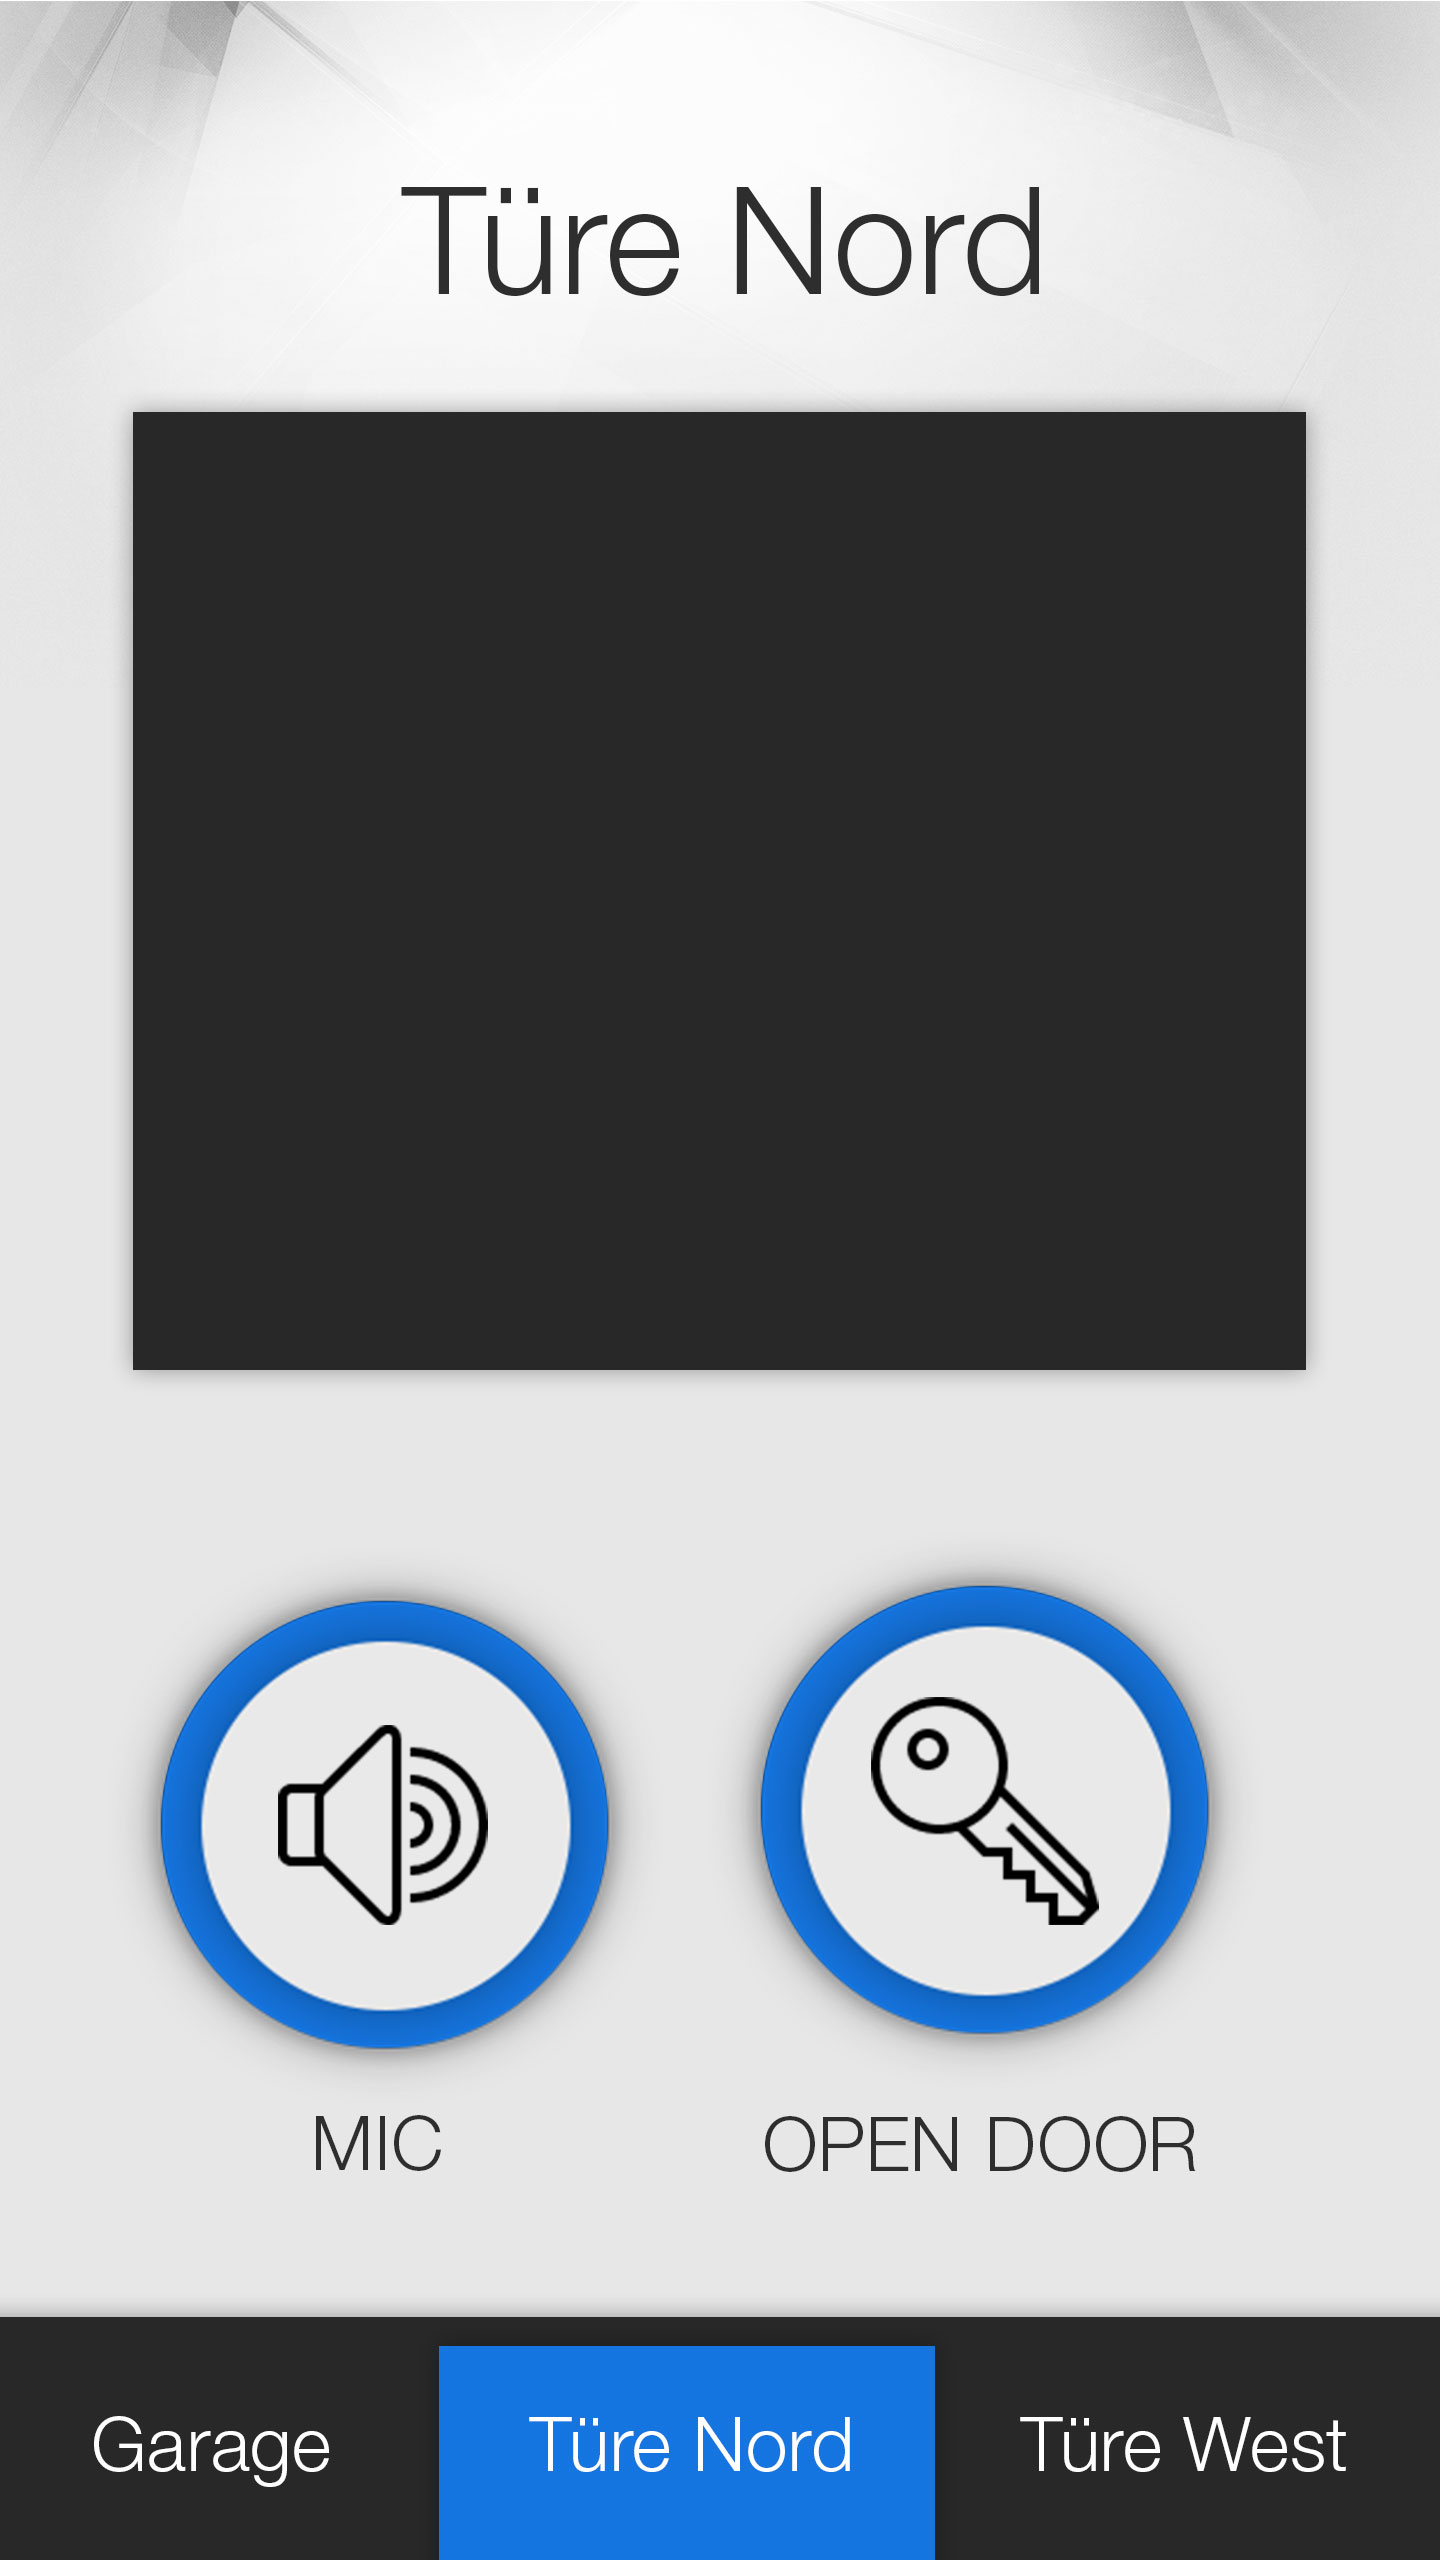
\includegraphics[width=0.35\textwidth]{clientDemo}
		\caption[Design der Client-Webapp]{Design der Client-Webapp}
		\label{fig:clientDemo}
	\end{center}
\end{figure}
\\
Die \cref{fig:clientDemo} zeigt das Design für die Webapplikation. Hier gezeigt ist die Smartphone Version. Dank ein Responsive-Design wird die selbe Applikation auch auf andere Geräte wie z.B. Tablets oder Computers passend angezeigt.
\\ 
Bei der Design-Entwurf standen Übersichtlichkeit und Benutzerfreundlichkeit im Vordergrund. Aus diesem Grund werden die Tasten für die Audio-Kommunikation und für die Öffnung der Türe gross Angezeigt. Das Videostream von der ausgewählte Türe wird sofort angezeigt und benötigt keine weitere Interaktion. 

\subsubsection{Aussensprechstelle Webapplikation}
..

\subsubsection{Management Tool}
\label{kap:managementtool}
Um eine schnellere Inbetriebnahme und eine zentrale Verwaltung des Systems zu gewährleisten, wurde der Management Tool etwickelt. Dieses Portal ermöglicht die Erfassung der Gegensprechanlagen und der Wohnungen.
Diese Schnitstelle wurde mit webtechnologien entwickelt(HTML, PHP, Js) und wird zusammen mit den MySQL Database auf den localen Raspberry Server gehostet. Aus Sicherheitsgründen werden alle eingehende und ausgehende Verbindungen abhörsicher aufgebaut.
\\
Grund dafür das einsetzten von Webtechnologien ist die Plattformunabhängigkeit sowie die Einfachkeit und die Standardisierung der Sprachen. Für den ersten Prototyp lag der Fokus auf die funktionale Eingenschaften der Tool. Bei einer zukünfitige Weiterentwicklung des Produkt kann man, dank der Webtechnologien mit gerigere Aufwand das Tool skalieren bzw. neue Features hinzufühgen.  

\begin{figure}[htb!]
	\begin{center}
		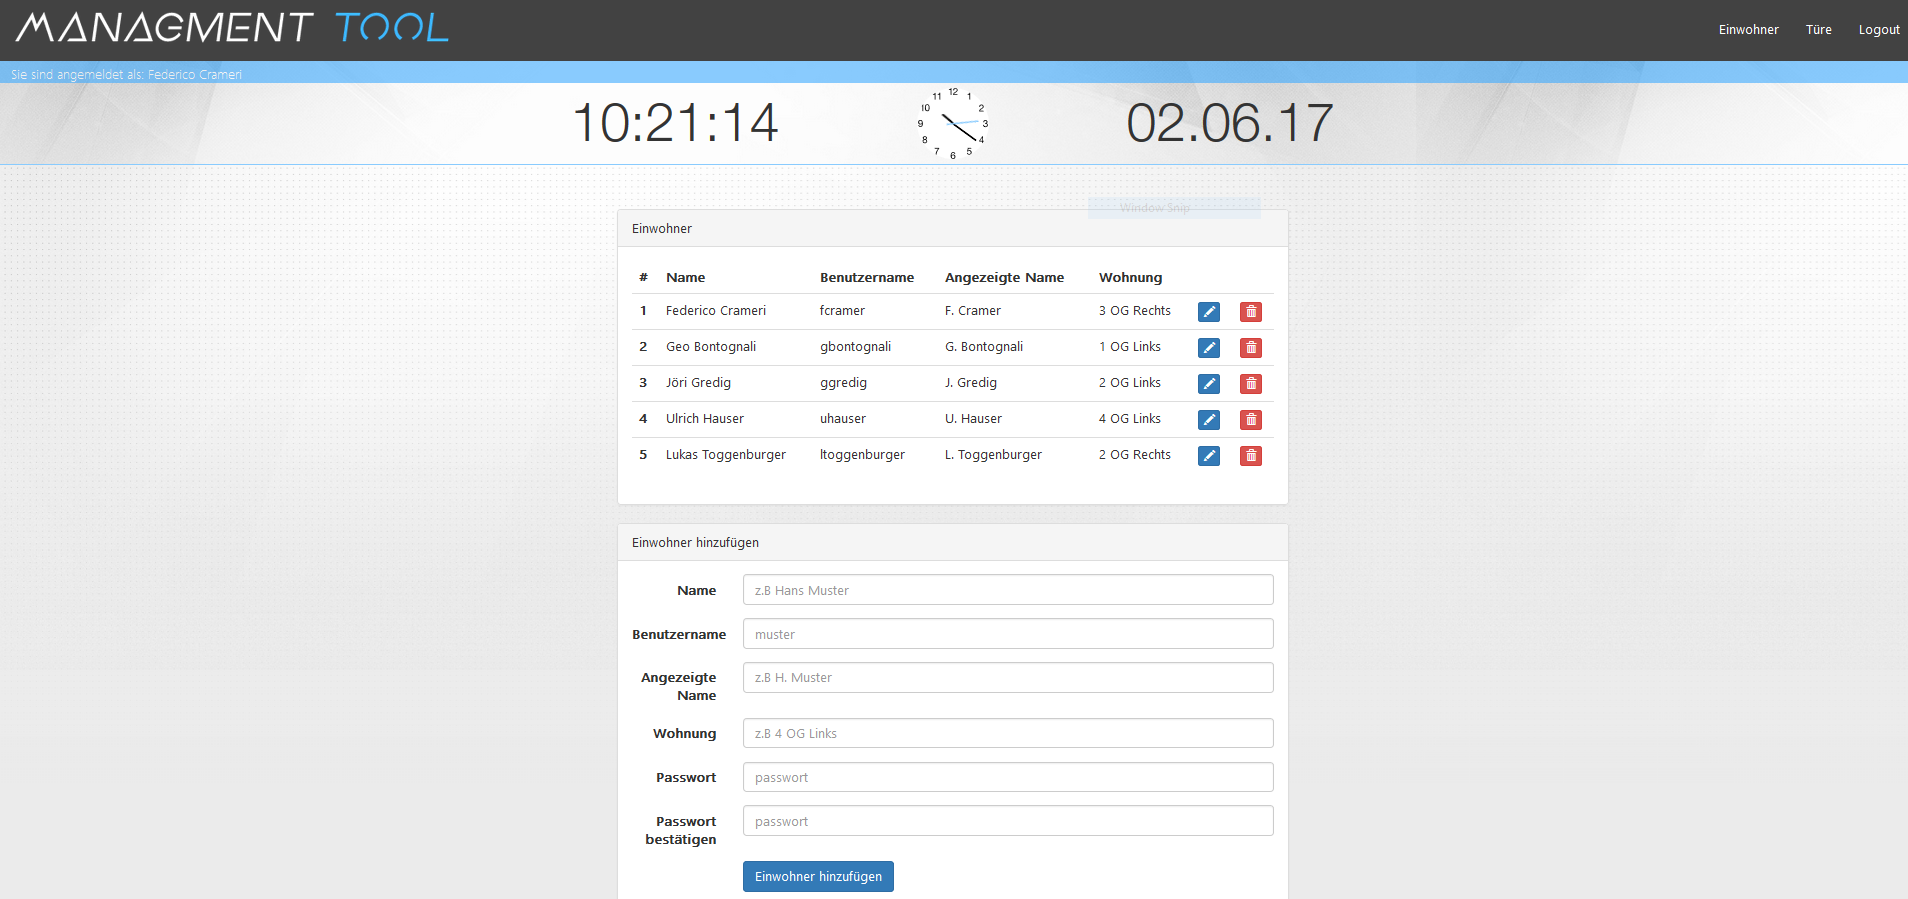
\includegraphics[width=1\textwidth]{managementtool}
		\caption[Design der Management tool]{Design der Management tool}
		\label{fig:managementtool}
	\end{center}
\end{figure}

Das Tool in mit ein Login versehen, somit ist sichergestellt das nur der Hausverwalter die Anlage verwalten kann. 
\subsubsection{Bewohner}
Unter die Bewohner Seite werden alle Wohnungen, beziehungsweise alle Bewohner aufgelistet. Diese verfühgen über ein Benutzername sowie eine Passwort die Von der Client App wervendet wird um sie sich bei den Server zu authentifizieren. Dieser Abschnitt bietet noch die Möglichkeit der Name und die Position der Wohnung welcher an den Aussensprechstelle ~\ref{fig:aussensprechstelle} angezeigt wird, abzuändern.
\subsubsection{Türen}
Bei der Einbau eine neue Tür, kann diese in dem Management Tool aufgeführt werden. Dabei muss beachtet werden dass der Id mit derjenige die auf den neu installierte Aussensprechstelle übereinstimmt. In diese Sektion sind auch die Namen der Türen definiert, welche denn auf den Client App (Siehe Abbildung ~\ref{fig:managementtool})  angezeigt werden. 


\subsection{Remote Verbindung}
\label{kap:remote}
..

\subsection{WebRTC}
\label{kap:webrtc}
WebRTC ist ein offener Standard, der eine Sammlung von Kommunikationsprotokollen und API beinhaltet. Die Standardisierung wird mehrheitlich betrieben und unterstützt von Google, Mozilla Foundation und Opera Software. WebRTC basiert auf HTML5 und Javascript und die Audio/Video Übertragung erfolgt über eine direkte Verbindung zwischen den Sprechpartner (Peer-to-Peer).
\\
\\
WebRTC wird hauptsächlich für die Entwicklung von Videokonferenz Programme verwendet. Die Natur dieses Projekt ist allerdings nicht dieselbe wie die herkömmliche Real-Time-Communication Applikationen. Glücklicherweise wurde WebRTC so entwickelt, um möglichst viel Flexibilität zu garantieren. Aus diesem Grund beinhaltet der WebRTC-Standard keine Definition für den Signaling-Process, welcher zusammen mit dem ICE (Interactive Connectivity Establishment) für den Verbindungsaufbau zwischen den Sprechpartnern zuständig ist. 

\begin{quote}
	\textit{
		"The thinking behind WebRTC call setup has been to fully specify and control the media plane, but to leave the signaling plane up to the application as much as possible. The rationale is that different applications may prefer to use different protocols, such as the existing SIP or Jingle call signaling protocols, or something custom to the particular application, perhaps for a novel use case. [...]"
	} 
	\\
	\cite[Sam Dutton, HTML5Rocks.com]{001} 
\end{quote}

\subsubsection{Signaling Process}
\label{kap:signaling}

Ähnlich wie bei VoIP-Telefonie \textit{(SIP)}, brauchen die Sprechpartner ein gemeinsam bekanntes Knoten, um die Verbindung zu initialisieren (\seeref{fig:signaling}). In den meisten Fällen ist einem Partner, die logische Adressierung der andere Partner nicht bekannt. Es besteht also keine Möglichkeit um eine P2P Verbindung auf einmal zu starten.
\begin{figure}[htb!]
	\begin{center}
		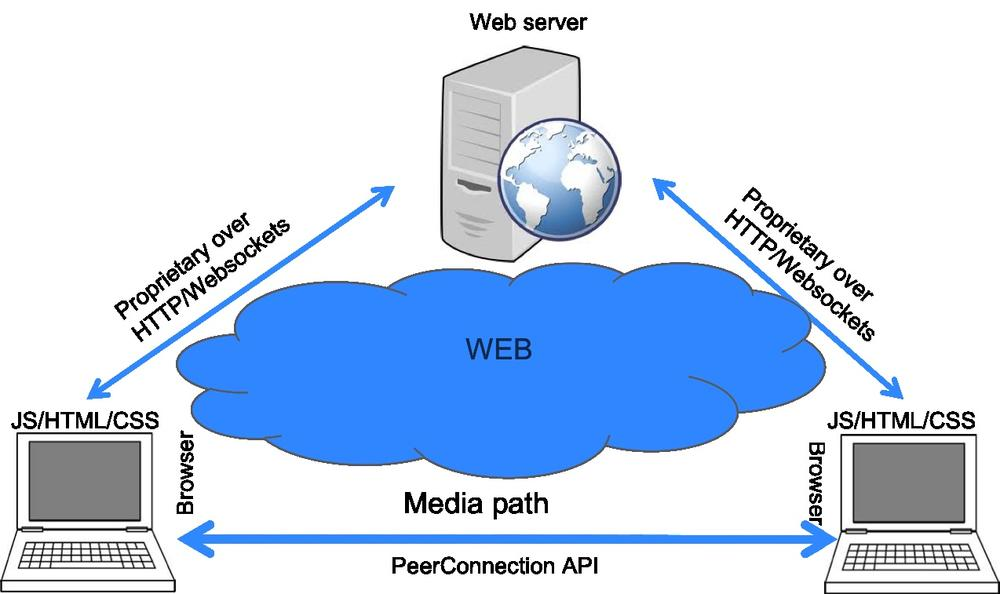
\includegraphics[width=0.75\textwidth]{signalingprocess}
		\caption[Der Signaling Prozess]{Der Signaling Prozess}
		\label{fig:signaling}
	\end{center}
\end{figure}
\\
Im unseren Fall wäre es theoretisch möglich, da die Position der Aussensprechstellen bzw. der Server immer dieselbe sind. Allerdings wurde WebRTC nicht so konzipiert. Die Standard WebRTC API beinhaltet kein Konstrukt um eine Verbindung anhand von Bekannter IP-Adresse aufbauen zu können.
\\
Im Internet sind es mehrere Signaling-Server Libraries verfügbar. Allerdings sind diese für andere Anwendungen gedacht. Im unseren System, wird beispielsweise nie eine Anruf von der Aussensprechstelle zu den Client-App gestartet, sondern lediglich umgekehrt.
\\
Für die Zwecke unser Projekt wurde ein eigenes Signaling-Server entwickelt. Dieser wird auf den Server ausgeführt und somit bleibt der Datenverkehr zwischen dem Client-App und der Aussensprechstelle, während jeder Schritt der Verbindungsaufbau und Kommunikation, innerhalb des lokales Netzwerkes. Das natürlich nur, solange der Bewohner sich zu Hause befindet.

\subsubsection{STUN Servers \& Remote Verbindung}
\label{test}
Eine Anforderung des Systems ist die Möglichkeit, auch ausserhalb des Heimnetzes mit den Aussensprechstellen sich verbinden zu können. Hier stellt das NAT-Protokoll (Network Adress Translation) ein Problem dar.
\\
Nach dem Signaling-Prozess wird das ICE-Prozess gestartet. Hier tauschen sich die zwei Partner Informationen über die eigene Adressierung und den \textit{best path} aus. Falls sich ein Sprechpartner hinter ein NAT-Knote befindet, wird für den anderen unmöglich sein eine Verbindung aufzubauen. Hier kommen die STUN-Servers im Spiel. Ähnlich wie bei dem Signalisierungsprozess stehen STUN-Servers als Hilfe für den Verbindungsaufbau da (\seeref{fig:stun}).
\begin{figure}[htb!]
	\begin{center}
		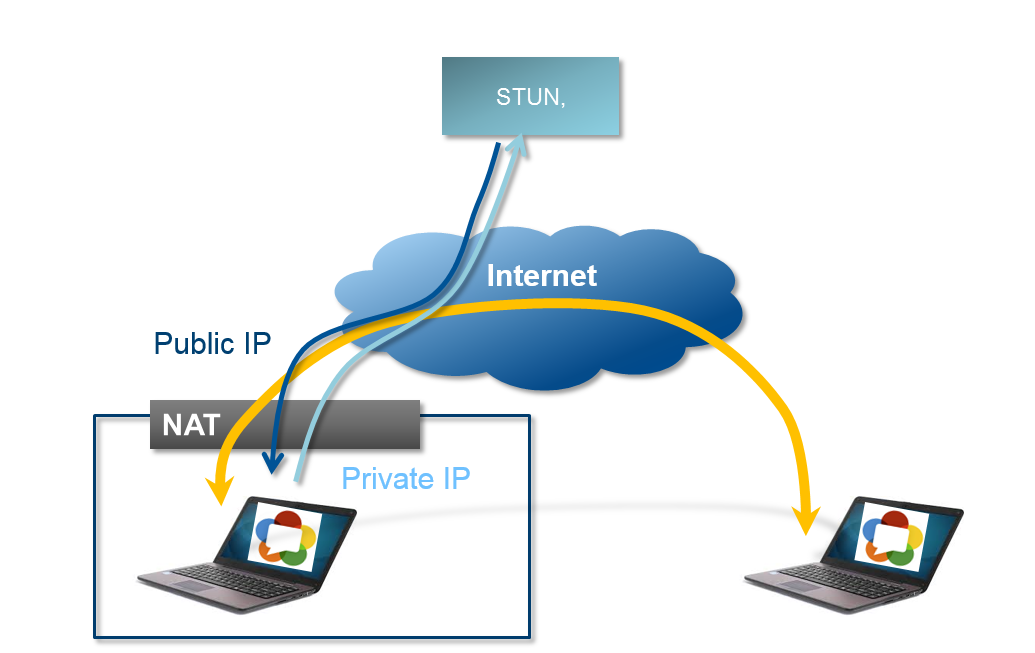
\includegraphics[width=0.75\textwidth]{stun}
		\caption[STUN Server]{STUN Server}
		\label{fig:stun}
	\end{center}
\end{figure}
 STUN-Servers informieren die Clients über jegliche NAT Konfigurationen die sich dazwischen befinden würden. Die beide Sprechpartner erhalten somit Informationen über welche Ports und Öffentliche Adressen die Verbindung initialisiert werden kann. Für die Entwicklung dieses Projektes werden die Google STUN Servers verwendet, welche kostenfrei zur Verfügung stehen.
\\
Falls sich beide Sprechpartner im gleichen lokales Netzwerk befinden, werden keine STUN-Servers benötigt und den gesamten Datenverkehr bleibt innerhalb des Heimnetzwerkes.

\newpage
\section{Testabnahme}
\label{sec:testabnahme}
Überprühfung der Anforderungen

\newpage
\section{Fazit und Ausblick}
\label{sec:fazit}
Der Fazit wir hier noch hinzugefühgt.
\newpage
\section{Anleitungen}
\label{sec:anleitungen}
Diese Anleitungen sind an dem zukünftigen Entwickler dieser Prototyp gerichtet. Mithilfe dieser Dokumentation und des mitgelieferten Images der Aussensprechstelle, soll ein Entwickler im Stand sein eine neu installierte Raspbian \gls{os} einer Aussensprechstelle/Server zu konfigurieren. Alles was konfiguriert wurde, wurde dokumentiert und in der Anleitung aufgeführt. Diese soll auch das Hinzufügen zukünftiger Funktionalitäten erleichtern.

\subsection{Aussensprechstelle Konfigurationsanleitung}

\subsubsection{Aktuelle Stand}
Betriebssystem:	Raspbian jessie with pixel\\
Version: April 2017\\
Kernel Version: 4.4

\subsubsection{Namen und Passwortkonzept}
Hostname: DoorPixxx (x= fortlaufende Nummerierung)\\
User: pi\\
Password: bachelor (Einfachheitshalber wurde dieses schwache Passwort ausgewählt. Sollte aber bei einer produktiven Inbetriebnahme zwingend geändert werden)\\

\subsubsection{Betriebssystem Installation}
\begin{itemize}
	\item Das Image von raspberry.com herunterladen und extrahieren \\ (https://www.raspberrypi.org/downloads/raspbian/)
	\item Um die Image auf der SD Karte zu bringen benutzt man Etcher.  (https://etcher.io/)
	\item Mit den Standard-Anmeldedaten Anmelden. User: pi Password: raspberry
\end{itemize}



\subsubsection{Allgemeine Einstellungen}
Das System soll auf dem neusten Stand aktualisieren werden
\begin{lstlisting}[backgroundcolor = \color{snippetcolor},
language = bash,
xleftmargin = 1cm,
framexleftmargin = 0.1em,
breaklines=true]
	apt-get update 
	sudo apt-get upgrade
\end{lstlisting}

Mit dem Terminalkommando ’sudo raspi-config’ können durch eine grafische Oberfläche folgende allgemeine Einstellungen angepasst werden:
\begin{itemize}
	\item Unter 'Interfacing Options' muss die SSH Server aktiviert werden.
	\item Hostname gemäss Namenskonzept anpassen
	\item Neue Passwort für den Pi Benutzer gemäss Password Konzept setzen.
	\item Zum Schluss sollen auch die Zeitzone, das Land und das Tastaturlayout angepasst werden.
\end{itemize}

\subsubsection{Bidschirm Konfiguration}
Die Displaytreiber von waveshare.com herunterladen und auf die SD Karte in Root Directory speichern. (http://www.waveshare.com/wiki/4inch\char`_HDMI\char`_LCD)\\
Mit folgenden Bash-Kommandos wird der Treiber installiert:
\begin{lstlisting}[backgroundcolor = \color{snippetcolor},
language = bash,
xleftmargin = 1cm,
framexleftmargin = 0.1em,
breaklines=true]
	tar xzvf /boot/LCD-show-YYMMDD.tar.gz 
	cd LCD-show/
	chmod +x LCD4-800x480-show
	./LCD4-800x480-show
\end{lstlisting}
Nachdem dass der Bildschirmtreiber installiert wurde, müssen die Einstellungen für den Bildschirm angepasst werden. Folgende Code-Zeilen müssen am Ende der ’config.txt’ Datei, die sich in der root-directory befindet, hinzugefügt werden \cite{displayConfig}.
\begin{lstlisting}[backgroundcolor = \color{snippetcolor},
language = bash,
xleftmargin = 1cm,
framexleftmargin = 0.1em,
breaklines=true]
	hdmi_group=2
	hdmi_mode=87
	hdmi_cvt 480 800 60 6 0 0 0
	dtoverlay=ads7846,cs=1,penirq=25,penirq_pull=2,
	speed=50000,keep_vref_on=0,swapxy=0,pmax=255,
	xohms=150,xmin=200,xmax=3900,ymin=200,ymax=3900
	display_rotate=3
\end{lstlisting}

\subsubsection{Browser Kiosk-mode}
Als erstes wird das Unclutter-Tool installiert um den Mausepfeil auszublenden.
\begin{lstlisting}[backgroundcolor = \color{snippetcolor},
language = bash,
xleftmargin = 1cm,
framexleftmargin = 0.1em,
breaklines=true]
	sudo apt-get install unclutter
\end{lstlisting}
Die Kiosk-Mode-Einstellungen werden in der config Datei  \\ (/home/pi/.config/lxsession/LXDE-pi/autostart) wie folgt angepasst
\begin{lstlisting}[backgroundcolor = \color{snippetcolor},
language = bash,
xleftmargin = 1cm,
framexleftmargin = 0.1em,
breaklines=true]
	# Chromium auto start in kiosk mode
	# path: /home/pi/.config/lxsession/LXDE-pi/autostart
	@lxpanel --profile LXDE-pi
	@pcmanfm --desktop --profile LXDE-pi
	#@xscreensaver -no-splash
	@point-rpi
	@xset s off
	@xset s noblank
	@xset -dpms
	@chromium-browser --noerrdialogs --kiosk --incognito https://172.16.111.99/server
\end{lstlisting}

\subsubsection{Aussensprechstelle Initialisierung}
Im Homeverzeichnis unter .config/autostart wird die Datei Aussensprechstelle.desktop erstellt.
\begin{lstlisting}[backgroundcolor = \color{snippetcolor},
language = bash,
xleftmargin = 1cm,
framexleftmargin = 0.1em,
breaklines=true]
	touch /home/pi/Aussensprechstelle/Startup/AussensprechstelleLauncher.sh
\end{lstlisting}
Inhalt des Scripst:
\begin{lstlisting}[backgroundcolor = \color{snippetcolor},
language = bash,
xleftmargin = 1cm,
framexleftmargin = 0.1em,
breaklines=true]
	#!/bin/bash
	# This script executes the needed commands on startup to initialize the Aussensprechstelle
	# /home/pi/Aussensprechstelle/Startup/AussensprechstelleLauncher.sh
	#
	# Activates the Camera Driver (Safe mode because of the chrome resolution bug)
	sudo modprobe bcm2835-v4l2 gst_v4l2src_is_broken=1
	#
	# Clears the old TasterController PID of the process (In case of system shutdown)
	file="/var/run/TasterController.pid"
	if [ -f $file ] ; then
		rm $file
	fi
	#
	# Starts the TasterController
	sudo java -jar /home/pi/Aussensprechstelle/TasterController/TasterController.jar &
	#
	# Creates the PID for the taster controller
	sudo echo $! > /var/run/TasterController.pid
	#
	# Starts the watchdog service
	sudo service watchdog start	
\end{lstlisting}

\subsubsection{Taster Controller}
Der Tastencontroller, der für den Key Mapping zuständig ist, wird vom oben gezeigten AussensprechstelleLauncher.sh unter /home/pi/Aussensprechstelle/TasterController/TasterController.jar gestartet. Die kompilierte Jar-Artefakt  muss also dorthin kopiert werden. 
\\
Folgende GPIO Pins werden von den 3 Tasten benötigt um die Aussensprechstelle zu steuern:
\begin{itemize}
	\item GPIO17(16) simuliert den Tastendruck J «Links navigieren»
	\item GPIO27(20) simuliert den Tastendruck K «Anrufen»
	\item GPIO22(21) simuliert den Tastendruck L «Rechts navigieren»
\end{itemize}

\subsubsection{Speaker Controller Service}
Als Erstes muss der mitgelieferte Jar Artefakt SpeakerController.jar unter folgenden Pfad kopiert werden:
\begin{lstlisting}[backgroundcolor = \color{snippetcolor},
language = bash,
xleftmargin = 1cm,
framexleftmargin = 0.1em,
breaklines=true]
	/home/door/Aussensprechstelle/SpeakerController/SpeakerController.jar
\end{lstlisting}
Um den Speaker-Controller als Service unter Unix laufen zu lassen, muss unter /etc/init.d/ das Speaker-Controller-Script erzeugt werden. Der Inhalt des Scripts wird mit dem Projekt mitgeliefert. Um es ausführbar zu machen, muss noch die
«execute» Berechtigung gegeben werden.

\begin{lstlisting}[backgroundcolor = \color{snippetcolor},
language = bash,
xleftmargin = 1cm,
framexleftmargin = 0.1em,
breaklines=true]
	touch /etc/init.d/speakerController
	chmod +x /etc/init.d/speakerController
\end{lstlisting}
Damit der SpeakerController-Service auch automatisch beim Systemstart ausgeführt wird, muss noch folgendes Kommando ausgeführt werden:
\begin{lstlisting}[backgroundcolor = \color{snippetcolor},
language = bash,
xleftmargin = 1cm,
framexleftmargin = 0.1em,
breaklines=true]
	sudo update-rc.d speakerController defaults
\end{lstlisting}
Der Speaker Controller kann nun mit folgenden Befehlen gestartet und gestoppt werden
\begin{lstlisting}[backgroundcolor = \color{snippetcolor},
language = bash,
xleftmargin = 1cm,
framexleftmargin = 0.1em,
breaklines=true]
	sudo service speakerController start
	sudo service speakerController stop
	sudo service speakerController restart
	sudo service speakerController status
\end{lstlisting}

\subsubsection{Watchdog/Watchdog deamon}
Um die von der Aussensprechstelle benötigte Dienste zu überwachen, wird ein Watchdog verwendet. Raspberry Pi hat ein «stad-alone» Hardware Watchdog die ein Autostart durchführt sobald eine der Dienste oder den OS still steht.
Mit folgenden Kommandos wird der Watchdog installiert:
\\
\begin{lstlisting}[backgroundcolor = \color{snippetcolor},
language = bash,
xleftmargin = 1cm,
framexleftmargin = 0.1em,
breaklines=true]
	sudo modprobe bcm2835-wdt
	sudo apt-get install watchdog chkconfig
	sudo chkconfig watchdog on
	sudo /etc/init.d/watchdog start
\end{lstlisting}
Damit die SpeakerController und die TasterController vom Watchdog überwacht werden, muss unter /etc/watchdog.conf die Konfigurationsdatei abgeändert werden. Der Inhalt der Konfigurationsdatei wird mit dem Projekt mitgeliefert.


\subsection{Server Konfigurationsanleitung}
\subsubsection{Aktuelle Stand}
Betriebssystem:	Raspbian jessie with pixel\\
Version: April 2017\\
Kernel Version: 4.4

\subsubsection{Namen und Passwortkonzept}
Hostname: SrvPixxx (x= fortlaufende Nummerierung)\\
User: pi\\
Password: raspberry (Default Password)\\


\subsubsection{Software Installation}
Nun werden die benötigten Dienste und Tools installiert, die vom Server benötigt werden.

\begin{itemize}
	\item Installation der Webserver. (PHP, Nginx, MySQL, Java SDK, Composer,
	Utils)
\end{itemize}

\begin{lstlisting}[backgroundcolor = \color{snippetcolor},
language = bash,
xleftmargin = 0.5cm,
framexleftmargin = 0.1em,
breaklines=true]
	apt-get install nginx
	udo apt-get install mysql-server
	apt-get install php5-fpm php5-mysql
	sudo apt-get install mysql-server mysql-client
	sudo apt-get install oracle-java8-jdk
	sudo apt-get install curl php5-cli git
	curl -sS https://getcomposer.org/installer | sudo php -- --install-dir=/usr/local/bin --filename=composer
\end{lstlisting}

\subsubsection{Erstellung SSL Zertifikate}
\label{kap:zertifikategen}
Bevor die Webapplikationen installiert werden können, müssen die Zertifikate generiert werden (Self-Signed).

\begin{itemize}
	\item Erstellung SSL Zertifikat für den Client Webapplikation. Als Hostname wird hier als Beispiel intercom.app verwendet. Zuerst muss eine Konfigurationsdatei (v3.ext) mit folgendem Inhalt generiert werden:
\end{itemize}

\begin{lstlisting}[backgroundcolor = \color{snippetcolor},
language = bash,
xleftmargin = 0.5cm,
framexleftmargin = 0.1em,
breaklines=true]
	authorityKeyIdentifier=keyid,issuer
	basicConstraints=CA:TRUE
	keyUsage = digitalSignature, nonRepudiation, keyEncipherment, dataEncipherment
	subjectAltName = @alt_names
	
	[alt_names]
	DNS.1 = intercom.app
\end{lstlisting}
Falls ein IP als hostname verwendet wird, kann man \texttt{@alt\_names} mit IP:192.168.0.18 ersetzen.

\begin{itemize}
	\item 
	Nun müssen folgende Befehle eingegeben werden. Wenn gefragt, muss der Hostname oder IP als Common Name (CN) eingegeben werden. Es kann immer das gleiche Passwort verwendet werden und muss dem Keystore-Password des Signaling-Servers entsprechen.
\end{itemize}

\begin{lstlisting}[backgroundcolor = \color{snippetcolor},
xleftmargin = 0.5cm,
framexleftmargin = 0.1em,
breaklines=true]
	sudo openssl genrsa -des3 -out rootCA.key 2048
	
	sudo openssl req -x509 -new -nodes -key rootCA.key -sha256 -days 1024 -out rootCA.pem
	
	sudo openssl req -new -sha256 -nodes -out server.csr -newkey rsa:2048 -keyout server.key
	
	sudo openssl x509 -req -in server.csr -CA rootCA.pem -CAkey rootCA.key -CAcreateserial -out server.crt -days 500 -sha256 -extfile v3.ext
	
	sudo openssl pkcs12 -export -in server.crt -inkey server.key -out cert.p12
	
	sudo keytool -importkeystore -srckeystore cert.p12 -srcstoretype PKCS12 -destkeystore keystore.jks -deststoretype JKS
	
	sudo openssl x509 -inform PEM -outform DER -in server.crt -out phone.der.crt

\end{lstlisting}

Somit wurden diverse Dateien generiert. Die folgenden werden später gebraucht.
\begin{itemize}
	\item server.cert und server.key -> SSL Zertifikate für Apache2
	\item rootCA.pem -> Root CA. Das muss in den Client-Browser importiert werden, damit die Clients den Server als vertraulich erkennen. 
	\item phone.der.crt -> Root CA für Mobilegeräte. Bei Mobilegeräte kann es per E-Mail verschickt werden und dann in die  Systemeinstellungen installiert werden.
	\item keystore.jks -> Das muss später in das selbe Verzeichnis kopiert werden, wo der SignalingServer installiert wird.  
\end{itemize}

\subsubsection{Konfiguration von Nginx}
Vor dem Deploy der Webapplikationen muss der Webserver noch konfiguriert werden.
\\
\begin{itemize}
	\item In der Datei /etc/php5/fpm/php.ini muss die folgende Zeile auskommentiert und editiert werden: 
\end{itemize}

\begin{lstlisting}[backgroundcolor = \color{snippetcolor},
language = bash,
xleftmargin = 0.5cm,
framexleftmargin = 0.1em,
breaklines=true]
	cgi.fix_pathinfo=0
\end{lstlisting}

\begin{itemize}
	\item 
	Nun muss Nginx so konfiguriert werden, dass PHP als compiler verwendet wird. Die Datei \textit{/etc/nginx/sites-available/default} muss editiert werden. Die Stellen die angepasst werden müssen sind rot markiert.
	\item 
	Nun müssen die zwei VirtualHosts für die zwei WebApps konfiguriert werden. Diese werden unter verschiedene Ports laufen. Dafür müssen zwei Konfigurationsdateien unter \textit{/etc/nginx/sites-available} erstellt werden. Bsp: intercom.app und management.app. Der Inhalt muss wie folgt aussehen. Die Stellen, die für die beiden Webapplikationen unterschiedlich sein müssen, sind rot markiert. Der Path zu den SSL-Zertifikate muss auch angepasst werden.
\end{itemize}

\begin{lstlisting}[backgroundcolor = \color{snippetcolor},
language = bash,
xleftmargin = 0.5cm,
framexleftmargin = 0.1em,
breaklines=true]
# Default server configuration
server {
# SSL configuration
listen 443 ssl;  # 444 for the second host
listen [::]:443 ssl;

ssl_certificate /path/to/the/certificate/server.crt;
ssl_certificate_key /path/to/the/certificate/server.key;

root /var/www/intercom/public;  # /management/public for the second host

# Add index.php to the list if you are using PHP
index index.php index.html index.htm index.nginx-debian.html;

server_name _;

location / {
# First attempt to serve request as file, then
# as directory, then fall back to displaying a 404.
try_files $uri $uri/ /index.php?$query_string;
}

location ~ \.php$ {
include snippets/fastcgi-php.conf;
fastcgi_pass unix:/var/run/php5-fpm.sock;
}
location ~ /\.ht {
deny all;
}
}
\end{lstlisting}

\begin{itemize}
	\item Zum abschliessen noch die folgenden Befehle eingeben:
\end{itemize}

\begin{lstlisting}[backgroundcolor = \color{snippetcolor},
language = bash,
xleftmargin = 0.5cm,
framexleftmargin = 0.1em,
breaklines=true]
sudo ln -s /etc/nginx/sites-available/intercom.app /etc/nginx/sites-enabled/
sud ln -s /etc/nginx/sites-available/management.app /etc/nginx/sites-enabled/
sudo service nginx reload
sudo service nginx restart
sudo service php5-fpm restart
sudo reboot

\end{lstlisting}

\subsubsection{Deploy Webapplikationen}
Vor dem Deploy der Webapplikationen muss der Webserver noch konfiguriert werden.
\\
\begin{itemize}
	\item Die beide Webapplikationen müssen zuerst auf dem Server in die passenden Verzeichnissen kopiert werden.\\
		/var/www/management\\
		/var/www/intercom
	\item Rechte anpassen
\end{itemize}

\begin{lstlisting}[backgroundcolor = \color{snippetcolor},
language = bash,
xleftmargin = 0.5cm,
framexleftmargin = 0.1em,
breaklines=true]
sudo chmod -R 775 /var/www
sudo chmod -R 777 /var/www/management/storage
sudo chmod -R 775 /var/www/intercom/storage
sudo chgrp -R www-data /var/www/
\end{lstlisting}

\begin{itemize}
	\item MySQL Database erstellen, dann Anmeldedaten und Database Name in der Datei: .env eingeben. (Falls .env nicht vorhanden: cp .env.example .env)
	\item Webapplikation installieren: (Diese Befehle müssen in der Root Dir jeder Webapp eingegeben werden).
\end{itemize}

\begin{lstlisting}[backgroundcolor = \color{snippetcolor},
language = bash,
xleftmargin = 0.5cm,
framexleftmargin = 0.1em,
breaklines=true]
composer install
php artisan migrate (MNGMT Tool Only)
php artisan key:generate
\end{lstlisting}
Die zwei Webapps müssten nun unter die ports 443 und 444 aufrufbar sein.

\subsubsection{Deploy Dienste und Services}
\begin{itemize}
	\item Zuerst die benötigten Pfade erstellen
\end{itemize}

\begin{lstlisting}[backgroundcolor = \color{snippetcolor},
language = bash,
xleftmargin = 0.5cm,
framexleftmargin = 0.1em,
breaklines=true]
mkdir /home/pi/server/signalingServer
mkdir /home/pi/server/relayController
\end{lstlisting}

\begin{itemize}
	\item Die beide kompilierte JARs in den entsprechenden Verzeichnissen kopieren. Die kompilierten JARs sind im jeweiligen Projektverzeichniss unter /deploy zu finden.
	\item Nun muss noch für den SignalingServer das vorher erstellte keystore.jks kopiert werden. Der Keystore muss sich im gleichen Verzeichnis wie der Signaling Server befinden.
	\item Für beide Dienste muss noch der \texttt{Autostart\_Skript} unter /etc/init.d/ kopiert werden. Die Skripte sind im Script-Verzeichnis gespeichert. Auch diese Skripte müssen ausführbar sein. Folgende Befehle müssen noch eingegeben werden:
\end{itemize}

\begin{lstlisting}[backgroundcolor = \color{snippetcolor},
language = bash,
xleftmargin = 0.5cm,
framexleftmargin = 0.1em,
breaklines=true]
sudo chmod +x /etc/init.d/signalingServer
sudo chmod +x /etc/init.d/relayController
sudo update-rc.d signalingServer defaults
sudo update-rc.d relayController defaults 
\end{lstlisting}



\subsection{Installation Client-Webapplikation}
\label{sec:clientappinst}
Es wird nun beschrieben, wie die Client-Webapplikation auf ein mobiles Gerät installiert werden kann.
Momentan wurde die Applikation hauptsächlich auf Android Smartphones mit Google Chrome getestet. Da es sich um eine Webapplikation handelt, ist das Betriebssystem von kleinerer Bedeutung. Wichtig ist, dass WebRTC vom Browser unterstützt wird.
\\
Die folgende Anleitung gilt für Android 7.0 Nougat. Die Installation wird auf andere Mobile Geräte auf jeden Fall nur leicht abweichen. 

\subsubsection{Installationsschritte}
\label{kap:clientappinst}
\textbf{Schritt 1: Installation der Zertifikate}
\begin{itemize}
	\item Die vorher generierte Mobile Zertifikat-Datei (\seeref{kap:zertifikategen}) auf das Smartphone kopieren. Das kann via USB oder E-Mail erfolgen. Wichtig ist, dass die Datei auf dem lokalen Speicher des Mobilgeräts vorhanden ist.
	\item Unter Options -> Security auf \textit{Install from  phone storage} klicken und die Zertifikat-Datei auswählen.
	\item Gerät neu starten.
\end{itemize}

\textbf{Schritt 2: Einbindung am Homescreen}
\\
Nun kann die Webapplikation bereits verwendet werden. Es reicht die folgende Adresse einzugeben: \textbf{https://SERVER/client?id=1}
\\
\textit{* SERVER -> Die IP Adresse oder Hostname des Servers.}
\\
\textit{** id=1 -> Diese ID definiert, welcher Einwohner sich gerade anmeldet. Welcher Einwohner zu welcher ID gehört, wird in dem Management Tool definiert. Wie in den \cref{kap:clientapp} bereits erwähnt, ist dies keine endgültige Lösung und nur für Vorführzwecke gedacht.}
\\
\\
Die Webapplikation besitzt ein \textit{Manifest-File}, welcher die Applikation als Standalone App konfigurieren kann. Um das zu aktivieren, muss die Webseite zur Homescreen hinzugefügt werden. Um das zu machen, auf das Overflow-Menü (drei kleine Punkte oben rechts) tippen und \textit{Zum Startbildschirm hinzufügen} auswählen.
\\
\\
Nun ist die Webapplikation als Standalone App verfügbar und kann somit auch in Fullscreen benutzt werden.


\section{Anhang}
\label{sec:anhang}

\subsection{Messungsresultate}
\label{ssec:resultate}
\begin{lstlisting}[backgroundcolor = \color{snippetcolor},
language = bash,
xleftmargin = 0.5cm,
framexleftmargin = 0.1em,
breaklines=true]
Switch#sh interfaces g0/43
GigabitEthernet0/43 is up, line protocol is up (connected)
Hardware is Gigabit Ethernet, address is 0023.05e2.c82b (bia 0023.05e2.c82b)
MTU 1500 bytes, BW 100000 Kbit/sec, DLY 100 usec,
reliability 255/255, txload 1/255, rxload 1/255
Encapsulation ARPA, loopback not set
Keepalive set (10 sec)
Full-duplex, 100Mb/s, media type is 10/100/1000BaseTX
input flow-control is off, output flow-control is unsupported
ARP type: ARPA, ARP Timeout 04:00:00
Last input never, output 00:00:00, output hang never
Last clearing of "show interface" counters never
Input queue: 0/75/0/0 (size/max/drops/flushes); Total output drops: 0
Queueing strategy: fifo
Output queue: 0/40 (size/max)
5 minute input rate 507000 bits/sec, 108 packets/sec
5 minute output rate 44000 bits/sec, 70 packets/sec
51357 packets input, 33613725 bytes, 0 no buffer
Received 130 broadcasts (82 multicasts)
0 runts, 0 giants, 0 throttles
0 input errors, 0 CRC, 0 frame, 0 overrun, 0 ignored
0 watchdog, 82 multicast, 0 pause input
0 input packets with dribble condition detected
32616 packets output, 6365458 bytes, 0 underruns
0 output errors, 0 collisions, 1 interface resets
0 unknown protocol drops
0 babbles, 0 late collision, 0 deferred
0 lost carrier, 0 no carrier, 0 pause output
0 output buffer failures, 0 output buffers swapped out
\end{lstlisting}

\subsection{Präsentation Prototyp}
\label{ssec:prototypfoto}
\begin{figure}[htb!]
	\begin{center}
		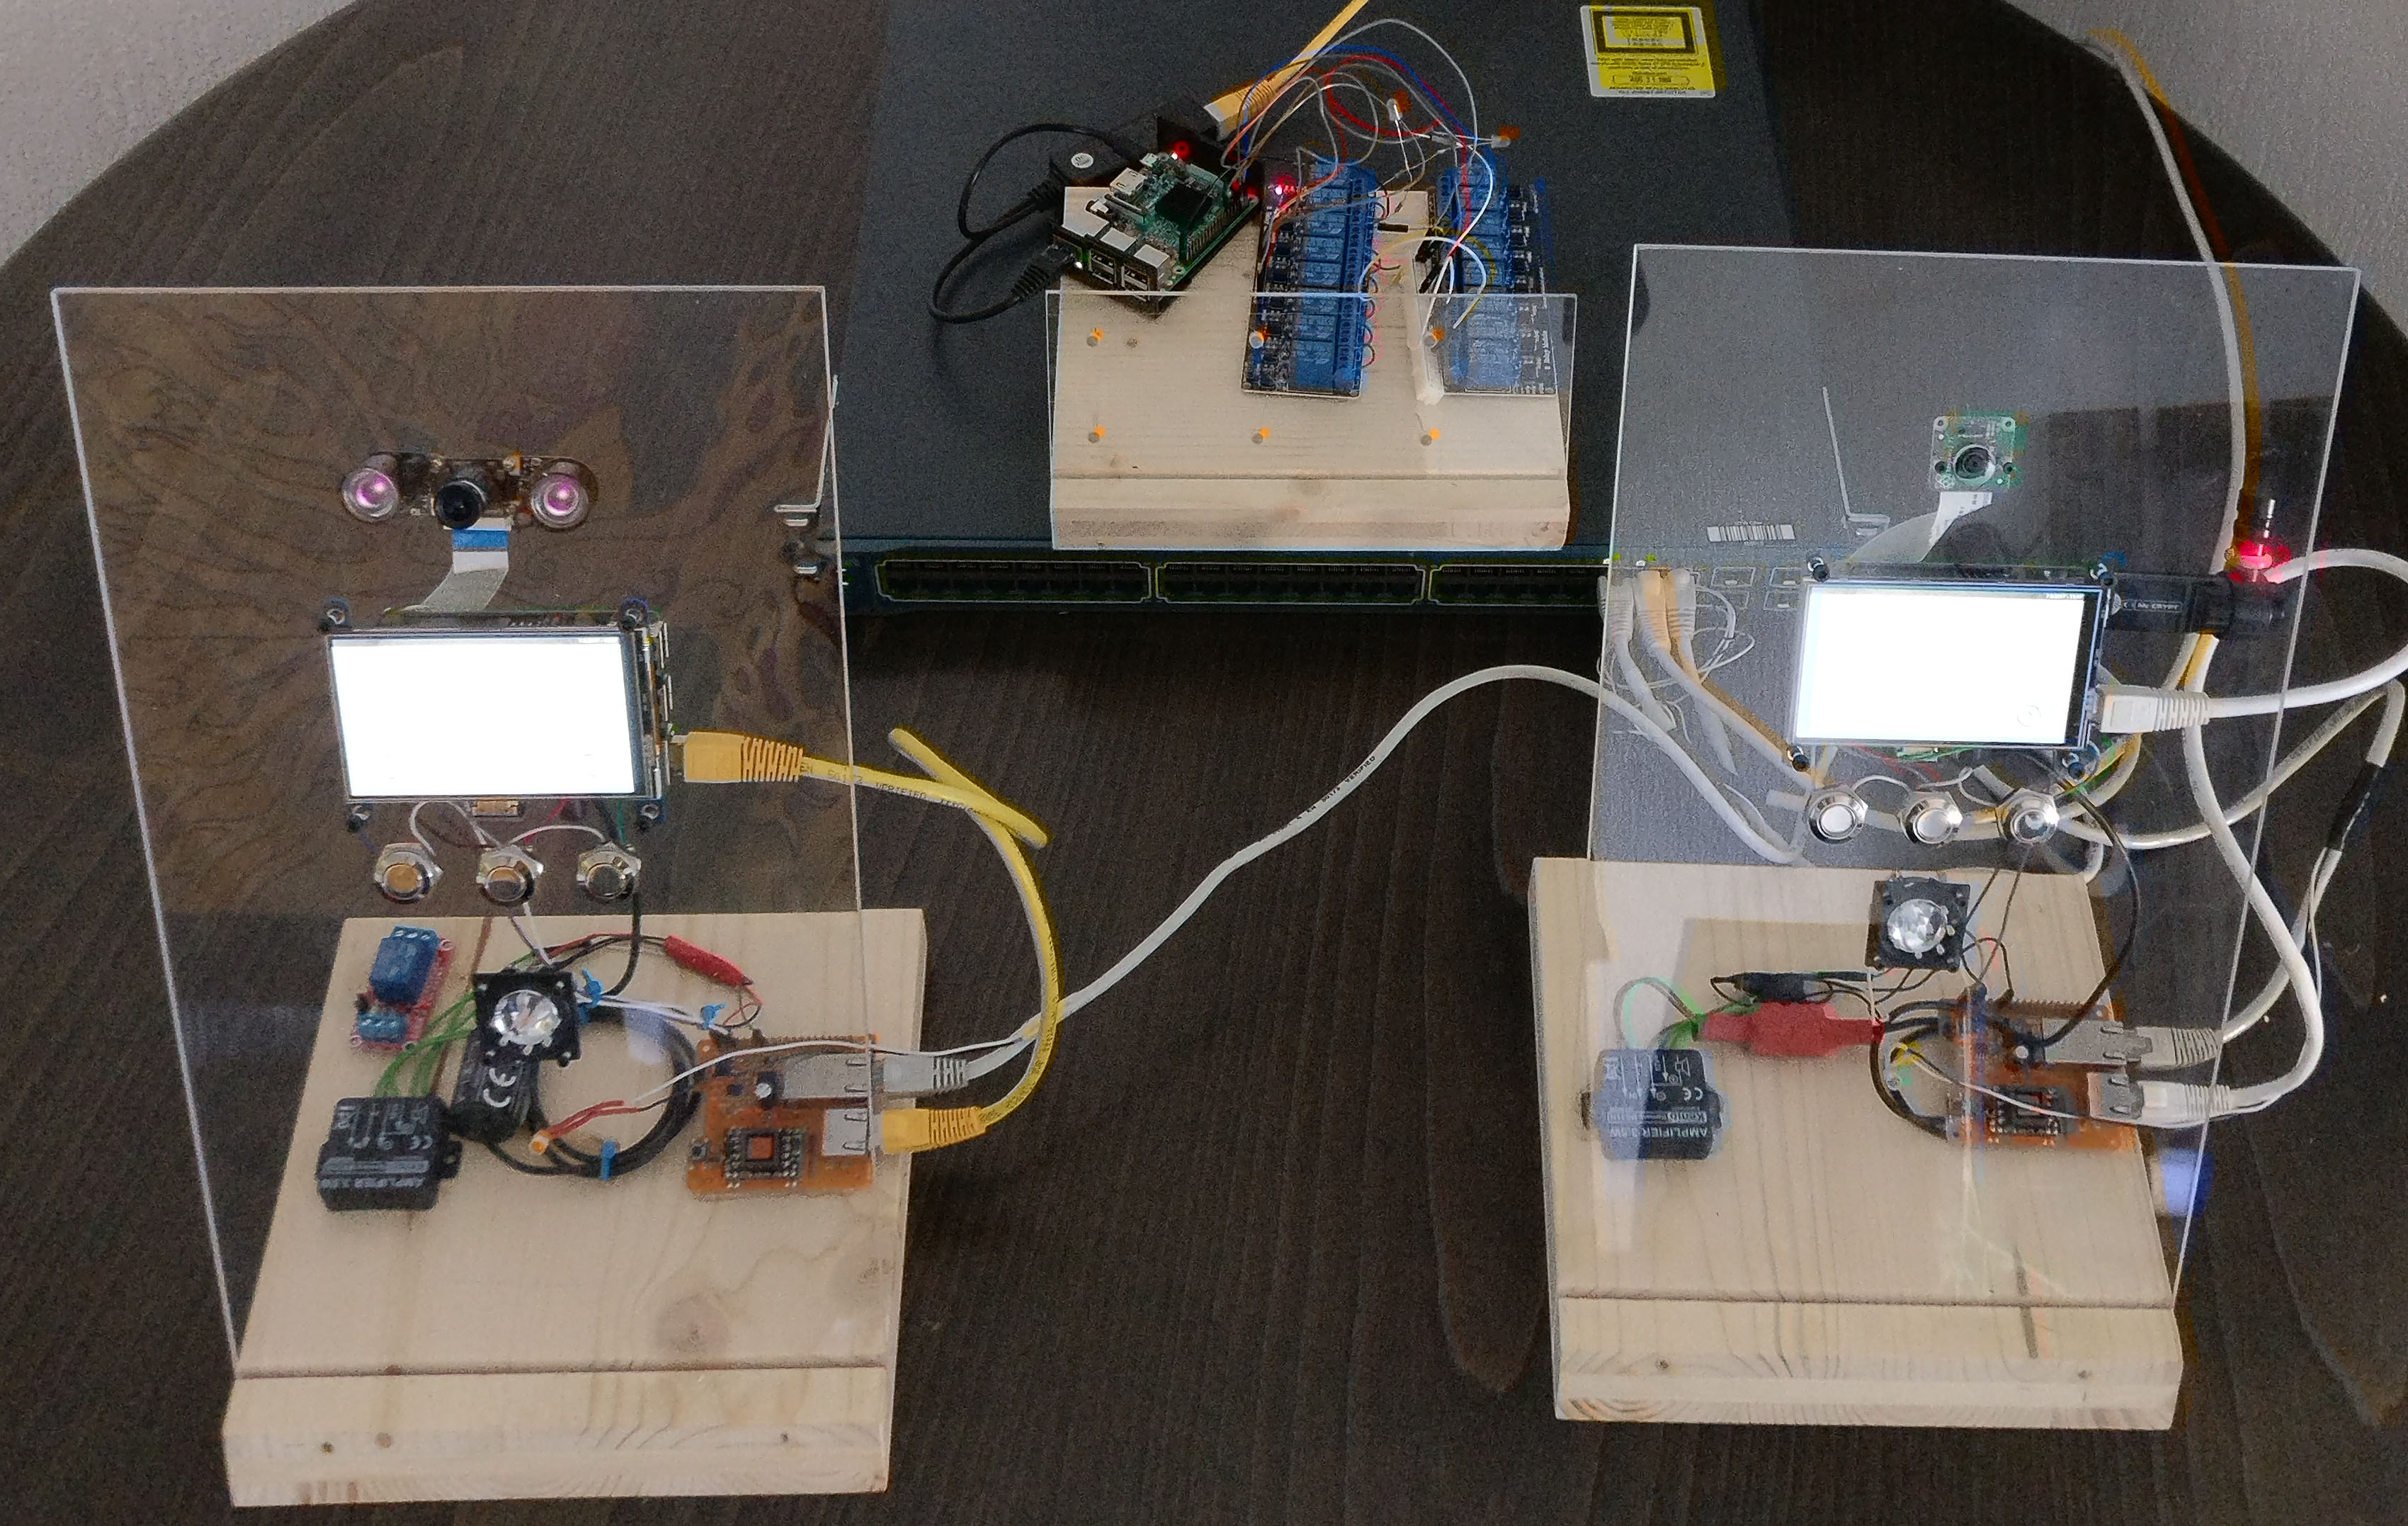
\includegraphics[width=0.95\textwidth]{prototyp}
		\caption[Prototyp Foto]{Präsentation Prototyp}
		\label{fig:prototyp}
	\end{center}
\end{figure}
\newpage















%%Verzeichnis aller Bilder






%% Abbildungsverzeichnis, Tabellenverzeichnis, Abkürzungsverzeichnis
\listoffigures
\addcontentsline{toc}{section}{Abbildungsverzeichnis}
\newpage
\listoftables
\addcontentsline{toc}{section}{Tabellenverzeichnis}


\newpage

\thispagestyle{plain}
\section*{Abkürzungsverzeichnis}
\addcontentsline{toc}{section}{Abkürzungsverzeichnis}
\newpage
\thispagestyle{plain}

%\begin{center}
%\begin{minipage}[t]{1\textwidth}
\section*{Eidesstattliche Erklärung}
\addcontentsline{toc}{section}{Eidesstattliche Erklärung}
Die Verfasser dieser Bachelorarbeit, Fabiano Sala und Gabriel Salkim, bestätigen, dass sie die Arbeit selbstständig und nur unter Benützung der angeführten Quellen und Hilfsmittel angefertigt haben. Sämtliche Entlehnungen sind durch Quellenangaben festgehalten.
	
	
\vspace{2cm}

\hspace{2cm} Ort, Datum \hfill Gabriel Salkim \hspace{2cm}

\vspace{4cm}

\hspace{2cm} Ort, Datum \hfill Fabiano Sala \hspace{2cm}
%\end{minipage}
%\end{center}






% leere Seite einfügen
\thispagestyle{empty}
\quad 
\newpage

%%Literaturverzeichnis
\nocite{*}
\printbibliography
%\printbibliography 


\end{document}
% ======================================= Dokumentende =======================================